\documentclass[11pt]{article}
\usepackage[margin=1in]{geometry}
\usepackage{amsmath,amssymb,amsthm}
\usepackage{booktabs}
\usepackage{tikz}
\usetikzlibrary{arrows.meta,decorations.markings}
\usepackage[colorlinks=true,linkcolor=blue!50!black,citecolor=green!40!black,urlcolor=blue!60!black]{hyperref}

\allowdisplaybreaks

% ---------------------------------------------------------------- environments
\theoremstyle{plain}
\newtheorem{theorem}{Theorem}[section]
\newtheorem{proposition}[theorem]{Proposition}
\newtheorem{lemma}[theorem]{Lemma}
\theoremstyle{definition}
\newtheorem{definition}[theorem]{Definition}
\newtheorem{example}[theorem]{Example}
\newtheorem{algo}{Algorithm}
\newtheorem{exercise}{Exercise}[section]
\theoremstyle{remark}
\newtheorem{remark}[theorem]{Remark}
\newtheorem*{physrem}{Physics remark (motivation only, may be skipped)}

\newenvironment{algobox}{\par\medskip\noindent\begin{minipage}{\linewidth}\hrule\smallskip}{\smallskip\hrule\end{minipage}\par\medskip}

% ---------------------------------------------------------------- notation
\newcommand{\Z}{\mathbb{Z}}
\newcommand{\Q}{\mathbb{Q}}
\newcommand{\R}{\mathbb{R}}
\newcommand{\C}{\mathbb{C}}
\newcommand{\PP}{\mathbb{P}}
\newcommand{\qn}[1]{[#1]}
\newcommand{\vu}{\mathbf{u}}
\newcommand{\vw}{\mathbf{w}}
\newcommand{\qrho}{q^{\rho}}
\newcommand{\qlr}[1]{q^{#1+\rho}}
\newcommand{\es}{\varnothing}
\newcommand{\tr}{{\mathsf t}}
\newcommand{\lt}[1]{#1^{\tr}}
\newcommand{\hatw}{\widehat{\omega}}
\newcommand{\topvertex}{\texttt{topvertex}}

% Young diagram: \yd{3,1}
\newcommand{\yd}[2][0.28]{\begin{tikzpicture}[scale=#1,baseline={(0,-0.6)}]
 \foreach \r [count=\i] in {#2} {\foreach \c in {1,...,\r} {\draw (\c-1,-\i+1) rectangle (\c,-\i);}}
\end{tikzpicture}}

\title{The topological vertex as an algorithm:\\ conventions and worked examples}
\author{Notes accompanying the Python package \texttt{topvertex}}
\date{}

\begin{document}
\maketitle

\begin{abstract}
We consider the topological string partition function $Z(q,Q)$ of a toric Calabi-Yau
threefold, which is specified by a picture: a triangulated lattice polygon. We explain how to
compute it by the topological vertex of Aganagic, Klemm, Mari\~no and Vafa, in the combinatorial
formulation of Konishi~\cite{Kon}, the conventions of which we follow. Nothing beyond linear
algebra, calculus and elementary combinatorics is assumed. Every object is defined before it is
used, and every rule is stated as an explicit algorithm with a worked example. Physics and
geometry appear only in separate remarks that can be skipped. In particular, we compute by hand
the first terms of $Z$ for the resolved conifold and for local $\PP^2$, and extract the first
Gopakumar-Vafa invariants $3,-6,27,\ldots$ of the latter. We also describe a comparison with
the Nekrasov partition functions of 5d linear quiver gauge theories. The notes accompany the
Python package \topvertex{}, which produced all the tables and all the formulas marked
``generated''.
\end{abstract}

\tableofcontents

%=====================================================================================
\section{Introduction and summary}\label{sec:intro}
%=====================================================================================

The Gopakumar-Vafa invariants $n^g_\beta$ of a Calabi-Yau threefold~\cite{GV} are among the most
studied invariants in enumerative geometry and string theory. For compact Calabi-Yau threefolds
they are very hard to compute. For toric ones, the topological vertex of Aganagic, Klemm,
Mari\~no and Vafa~\cite{AKMV} computes all of them, in every genus, by finite combinatorics (see
\cite{Marino} for a review). In these notes we consider the topological vertex as an algorithm.
We follow the formulation of Konishi~\cite{Kon}, in which the input is a lattice polygon and
every intermediate quantity is an explicit rational function.

The input is a \textit{picture}: a convex polygon in the plane with corners at integer points,
cut into small triangles with corners again at integer points (the precise definitions are
given in Section~\ref{sec:polygons}). The three pictures that we will use most are the
following:
\begin{center}
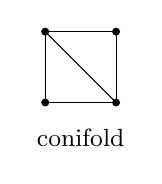
\begin{tikzpicture}[scale=0.9]
 \foreach \p in {(0,0),(1,0),(0,1),(1,1)} \fill \p circle (1.6pt);
 \draw (0,0)--(1,0)--(1,1)--(0,1)--cycle; \draw (1,0)--(0,1);
 \node at (0.5,-0.5) {\small conifold};
\end{tikzpicture}\qquad\qquad
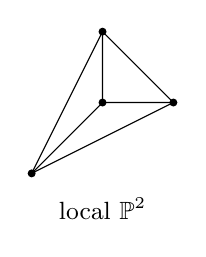
\begin{tikzpicture}[scale=0.9]
 \foreach \p in {(0,0),(1,0),(0,1),(-1,-1)} \fill \p circle (1.6pt);
 \draw (1,0)--(0,1)--(-1,-1)--cycle; \draw (0,0)--(1,0) (0,0)--(0,1) (0,0)--(-1,-1);
 \node at (0,-1.5) {\small local $\PP^2$};
\end{tikzpicture}\qquad\qquad
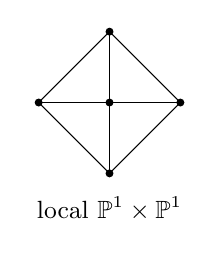
\begin{tikzpicture}[scale=0.9]
 \foreach \p in {(0,0),(1,0),(0,1),(-1,0),(0,-1)} \fill \p circle (1.6pt);
 \draw (1,0)--(0,1)--(-1,0)--(0,-1)--cycle; \draw (1,0)--(-1,0) (0,1)--(0,-1);
 \node at (0,-1.5) {\small local $\PP^1\times\PP^1$};
\end{tikzpicture}
\end{center}
The output is a formal power series
\begin{equation}\label{eq:Zintro}
Z(q;Q)=1+\sum_{\mathbf d\neq 0} Z_{\mathbf d}(q)\,Q^{\mathbf d},\qquad
Q^{\mathbf d}=\prod_e Q_e^{d_e},
\end{equation}
with one variable $Q_e$ for every \textit{interior} segment $e$ of the triangulation, that is
for every segment that is not on the boundary of the polygon. The coefficients
$Z_{\mathbf d}(q)$ are \textit{rational functions} of $q^{1/2}$. From $Z$ one passes to the free
energy $F=\log Z$ and then to a table of \textit{integers} $n^g_\beta$, the Gopakumar-Vafa
invariants, labelled by a ``degree'' $\beta$ and a ``genus'' $g\ge 0$. For example, the first
ones for local $\PP^2$ are $n^0_1=3$, $n^0_2=-6$, $n^0_3=27$, $n^1_3=-10$. We will compute the
first two of these by hand.

\begin{physrem}
A triangulated lattice polygon describes a \textit{toric Calabi-Yau threefold} $X$. It is a
non-compact complex manifold of complex dimension three, built by gluing copies of $\C^3$, one
for each small triangle. Interior segments correspond to holomorphic spheres $\PP^1\subset X$,
and $Q_e=e^{-t_e}$, where $t_e$ (a \textit{K\"ahler parameter}) is the area of that sphere. The
free energy $F=\log Z$ is the generating function of the Gromov-Witten invariants, the
``numbers'' of holomorphic maps from Riemann surfaces of every genus into $X$. The
Gopakumar-Vafa reorganization turns these rational numbers into integers $n^g_\beta$ that count
BPS states of M-theory~\cite{GV}. The rule that computes $Z$ is the \textit{topological vertex}
of~\cite{AKMV}. It was derived from Chern-Simons theory (see \cite{Marino} for a review) and
proved mathematically in~\cite{LLLZ}. We follow the purely combinatorial formulation
of~\cite{Kon}, where it was used to prove that the $n^g_\beta$ are integers.
\end{physrem}

The whole computation is summarized in Algorithm~\ref{alg:overview} below. Every word in it
will be defined in Sections~\ref{sec:polygons}-\ref{sec:classes}.

\begin{algobox}
\setcounter{algo}{-1}
\begin{algo}[The topological vertex, overview]\label{alg:overview}\ \\
\textbf{Input:} a convex lattice polygon with a regular unimodular triangulation, and a
truncation degree $D$.\\
\textbf{Output:} the coefficients of $Z(q;Q)$ up to degree $D$, the free energy $F=\log Z$, and
the Gopakumar-Vafa integers $n^g_\beta$ up to degree $D$.
\begin{enumerate}
\item \textit{Graph.} Put one node $v_\sigma$ in each small triangle $\sigma$, one edge $e_\tau$
across each interior segment $\tau$, and one outgoing ray across each boundary segment
(Section~\ref{ssec:dual}).
\item \textit{Framings.} For each interior segment $\tau$ compute an integer $n_\tau$ (its
framing) from the four lattice points of the two triangles containing $\tau$, after choosing a
direction for $e_\tau$ (Section~\ref{ssec:framing}).
\item \textit{Sum over partitions.} Attach a partition $\lambda_\tau$ (a Young diagram) to every
interior segment, and add up
\begin{equation}
\prod_\tau (-1)^{|\lambda_\tau|(n_\tau+1)}\,q^{n_\tau\kappa(\lambda_\tau)/2}\,
Q_\tau^{|\lambda_\tau|}\;\prod_\sigma C_{\lambda_\sigma}(q)
\end{equation}
over all choices with $\sum_\tau w_\tau|\lambda_\tau|\le D$. Here $|\lambda|$ is the number of
boxes of $\lambda$, and $\kappa(\lambda)$ is an even integer that is quadratic in the row
lengths of $\lambda$. Namely, it is the $N$-independent part of the quadratic Casimir
$\kappa(\lambda)+N|\lambda|$ of the representation of $U(N)$ labelled by $\lambda$, and its
explicit form is given in (\ref{eq:kappa}). The function $C_{\lambda\mu\nu}(q)$ is the
\textit{topological vertex}, an explicit rational function of $q^{1/2}$ built from Schur
functions (Section~\ref{sec:vertex}), and $\lambda_\sigma$ is the triple of partitions around
the triangle $\sigma$ (Section~\ref{ssec:gluing}). The positive integers $w_\tau$ are the
\textit{weights} of the interior segments. They are determined by \textit{heights} of the
triangulation, that is by numbers attached to the lattice points such that the triangulation is
the projection of the lower convex hull of the lifted points (Section~\ref{ssec:heights}).
\item \textit{Curve classes.} Replace each $Q_\tau$ by a monomial in independent variables
according to the ``class'' of $\tau$ (Section~\ref{sec:classes}).
\item \textit{Free energy and integers.} Take $F=\log Z$ and peel off multiple covers to obtain the
integers $n^g_\beta$ (Section~\ref{sec:gv}).
\end{enumerate}
\end{algo}
\end{algobox}

The output of Algorithm~\ref{alg:overview} can be compared with independent computations. One
comparison is provided by the tables of invariants in~\cite{CKYZ,KKV}, some of which are
reproduced in Table~\ref{tab:gv}. Another one is available for the ``ladder'' polygons of
Appendix~\ref{app:nekrasov}, for which $Z$ is related to the Nekrasov instanton partition
function of a 5d gauge theory~\cite{Nekrasov,IKP-SUN}.

Throughout the notes, unless explicitly mentioned otherwise, we use the conventions
of~\cite{Kon}, which are also those of the package \topvertex{} (file \texttt{CONVENTIONS.md}). In
particular, we write
\begin{equation}
x=q^{1/2},\qquad [k]=q^{k/2}-q^{-k/2}=x^k-x^{-k},
\end{equation}
so that rational functions of $q^{1/2}$ are rational functions of $x$. The vertex is the one of
Definition~\ref{def:vertex}, the framings are as in Definition~\ref{def:framing}, and the
Gopakumar-Vafa expansion is (\ref{eq:GV}). Other papers use other conventions, and
Appendix~\ref{app:conventions} is a dictionary. Formulas and tables labelled ``generated'' are
\verb|\input| from the directory \texttt{notes/generated/}, which is written by the script
\texttt{notes/make\_tables.py} calling the package. Everything else was computed by hand and
checked against the package.

The rest of the notes is organized as follows. In Section~\ref{sec:polygons} we describe the
input: lattice polygons, unimodular triangulations, the dual graph, and the heights of a
regular triangulation. In Sections~\ref{sec:partitions} and~\ref{sec:schur} we review
partitions, $q$-numbers and Schur functions, which is everything needed for the vertex
$C_{\lambda\mu\nu}$ defined in Section~\ref{sec:vertex}. In Section~\ref{sec:gluing} we define
the framings and state the gluing rule (\ref{eq:Z}) for the partition function. In
Section~\ref{sec:examples} we work out the resolved conifold, local $\PP^2$ and local
$\PP^1\times\PP^1$ by hand. In Section~\ref{sec:gv} we extract the Gopakumar-Vafa invariants
from the free energy. Finally, in Section~\ref{sec:classes} we explain curve classes and how to
truncate the sum over partitions consistently. The appendices contain the comparison with the
Nekrasov partition function of a linear quiver (Appendix~\ref{app:nekrasov}), a dictionary
between our conventions and those of the literature (Appendix~\ref{app:conventions}), and the
answers to the exercises (Appendix~\ref{app:answers}).

%=====================================================================================
\section{Lattice polygons and their triangulations}\label{sec:polygons}
%=====================================================================================

In this section we describe the input of Algorithm~\ref{alg:overview}: a convex lattice polygon,
a unimodular triangulation of it, the dual graph, and the heights of the triangulation.


\subsection{Lattice points, polygons, unimodular triangles}

\begin{definition}
A \textit{lattice point} is a point $\omega=(a,b)\in\R^2$ with $a,b\in\Z$. A \textit{convex lattice
polygon} $P$ is the convex hull of finitely many lattice points, not all on a line. Its
\textit{corners} are the points of $P$ that are not in the middle of a segment contained in $P$,
and they are lattice points. A lattice point of $P$ is a \textit{boundary point} if it lies on the
boundary of $P$ and an \textit{interior point} otherwise. We write $I$ and $B$ for the numbers of
interior and boundary lattice points.
\end{definition}

For three points $\omega_1,\omega_2,\omega_3$ in the plane put
\begin{equation}\label{eq:det}
\det(\omega_1,\omega_2,\omega_3):=\det\begin{pmatrix}a_2-a_1 & a_3-a_1\\ b_2-b_1& b_3-b_1\end{pmatrix},
\qquad \omega_i=(a_i,b_i).
\end{equation}
This is \textit{twice the signed area} of the triangle with corners
$\omega_1,\omega_2,\omega_3$. It is positive exactly when the corners are listed
\textit{counterclockwise} (ccw). It is also equal to the $3\times 3$ determinant
\begin{equation}\label{eq:det3}
\det(\omega_1,\omega_2,\omega_3)=\det\begin{pmatrix}a_1&a_2&a_3\\ b_1&b_2&b_3\\ 1&1&1\end{pmatrix},
\end{equation}
as one sees by subtracting the first column from the other two. We will use the column vectors
$\hatw_i=(a_i,b_i,1)$ repeatedly.

\begin{definition}
A lattice triangle (its corners are lattice points, not on a line) is
\textit{unimodular} if $|\det(\omega_1,\omega_2,\omega_3)|=1$, i.e.\ if its area is $1/2$, the
smallest possible.
\end{definition}

\begin{theorem}[Pick]
For a convex lattice polygon, $\operatorname{Area}(P)=I+\tfrac{B}{2}-1$.
\end{theorem}

\begin{lemma}\label{lem:unimodular}
A lattice triangle is unimodular if and only if its only lattice points are its three corners.
Equivalently, the three vectors $\hatw_1,\hatw_2,\hatw_3$ form a basis of $\Z^3$ (every integer
vector is an integer combination of them).
\end{lemma}
\begin{proof}
By the Pick theorem, the area $1/2$ means $I+B/2=3/2$. Since $B\ge3$, this forces $B=3$ and
$I=0$, and conversely.
The second statement holds because an integer matrix has an integer inverse if and only if its determinant
is $\pm1$, and the determinant is (\ref{eq:det3}).
\end{proof}

\begin{example}
$(0,0),(1,0),(0,1)$ is unimodular ($\det=1$, ccw). $(0,0),(2,0),(0,1)$ is not ($\det=2$, and it
contains the extra lattice point $(1,0)$).
\end{example}

\subsection{Unimodular triangulations}

\begin{definition}
A \textit{unimodular triangulation} of a convex lattice polygon $P$ is a finite set of unimodular
lattice triangles with the following properties: (i) their union is $P$, (ii) two different
triangles meet in a common side, a common corner, or not at all, (iii) \textit{every} lattice
point of $P$ is a corner of some triangle. The sides of the triangles are called
\textit{segments}. A segment is \textit{interior} if
it is not contained in the boundary of $P$ (then exactly two triangles contain it), and a
\textit{boundary segment} otherwise (then exactly one triangle contains it).
\end{definition}

\begin{lemma}\label{lem:counting}
A unimodular triangulation of $P$ has $T=2\operatorname{Area}(P)=2I+B-2$ triangles, $B$ boundary
segments and $E=3I+B-3$ interior segments.
\end{lemma}
\begin{proof}
Each triangle has area $1/2$, which gives $T$ (and Pick gives the second expression). The
boundary is cut into $B$ segments by its $B$ lattice points. Counting pairs (triangle, side) in
two ways gives $3T=2E+B$, so that $E=(3T-B)/2=3I+B-3$.
\end{proof}

\begin{example}\label{ex:three}
The three basic examples of these notes (Figure~\ref{fig:webs}):
\begin{itemize}
\item \textit{Conifold}: the unit square with corners $(0,0),(1,0),(1,1),(0,1)$, cut by the
diagonal from $(1,0)$ to $(0,1)$. $I=0$, $B=4$: two triangles, one interior segment.
\item \textit{Local $\PP^2$}: the triangle with corners $(1,0),(0,1),(-1,-1)$ and the center
$(0,0)$. Here $I=1$, $B=3$ and the area is $3/2$: three triangles and three interior segments (from the center
to the corners). This is the unique unimodular triangulation, since all lattice points must be
used.
\item \textit{Local $\PP^1\times\PP^1$} (also called local $F_0$): the ``diamond'' with corners
$(1,0),(0,1),(-1,0),(0,-1)$ and center $(0,0)$. Here $I=1$, $B=4$: four triangles and four interior
segments.
\end{itemize}
\end{example}

\subsection{The dual graph and its \texorpdfstring{$(p,q)$}{(p,q)}-vectors}\label{ssec:dual}

\begin{definition}[Dual graph, or web]\label{def:dual}
Given a unimodular triangulation, its \textit{dual graph} $\Gamma$ has
\begin{itemize}
\item one \textit{node} $v_\sigma$ for every triangle $\sigma$,
\item one \textit{internal edge} $e_\tau$ for every interior segment $\tau$, joining the nodes of
the two triangles that contain $\tau$,
\item one \textit{external leg} (a half-infinite ray starting at $v_\sigma$) for every boundary
segment of $\sigma$.
\end{itemize}
Every node has exactly three \textit{legs} (internal edges or external legs), one through each
side of its triangle.
\end{definition}

The dual graph can be drawn with straight edges in a canonical way. For a triangle $\sigma$
with corners listed counterclockwise, $(\omega_a,\omega_b,\omega_c)$, the three sides
\textit{in counterclockwise order} are $\omega_a\rightarrow\omega_b$, $\omega_b\rightarrow\omega_c$,
$\omega_c\rightarrow\omega_a$. To the side $\omega_a\rightarrow\omega_b$ with direction vector
$d=\omega_b-\omega_a=(d_1,d_2)$ we attach the vector
\begin{equation}\label{eq:pq}
v=(d_2,-d_1)\qquad(\text{$d$ rotated by $-90^\circ$}).
\end{equation}
Because the corners are ccw, $v$ is the \textit{outward normal} of that side. These are the
\textit{$(p,q)$-vectors} of the three legs at $v_\sigma$: the leg through a side is drawn in the
direction of $v$.

\begin{lemma}[Balancing]
At every node the three $(p,q)$-vectors add up to zero, and consecutive ones (in ccw order)
satisfy $\det(v,v')=v_1v'_2-v_2v'_1=+1$. If $\tau$ is an interior segment, the vectors attached
to $\tau$ by its two triangles are opposite.
\end{lemma}
\begin{proof}
The three side vectors of a triangle add to zero, and (\ref{eq:pq}) is linear. Rotation
preserves determinants, and for consecutive ccw sides $\det(\omega_b-\omega_a,\omega_c-\omega_b)
=\det(\omega_a,\omega_b,\omega_c)=1$. The two triangles containing $\tau$ traverse it in opposite
directions.
\end{proof}

\begin{example}
For $\sigma=\{(0,0),(1,0),(0,1)\}$ (ccw in this order) the sides are $(1,0)$, $(-1,1)$,
$(0,-1)$ and the legs are $v=(0,-1)$ (down), $(1,1)$ (up-right), $(-1,0)$ (left): their sum
is $0$.
\end{example}

Therefore the dual graph is a planar trivalent graph with edges perpendicular to the segments they
cross. It is called the \textit{web} or \textit{toric diagram}. Figure~\ref{fig:webs} shows the three
examples. The arrows and numbers on the internal edges will be explained in
Section~\ref{sec:gluing}.

\begin{figure}[ht]
\centering
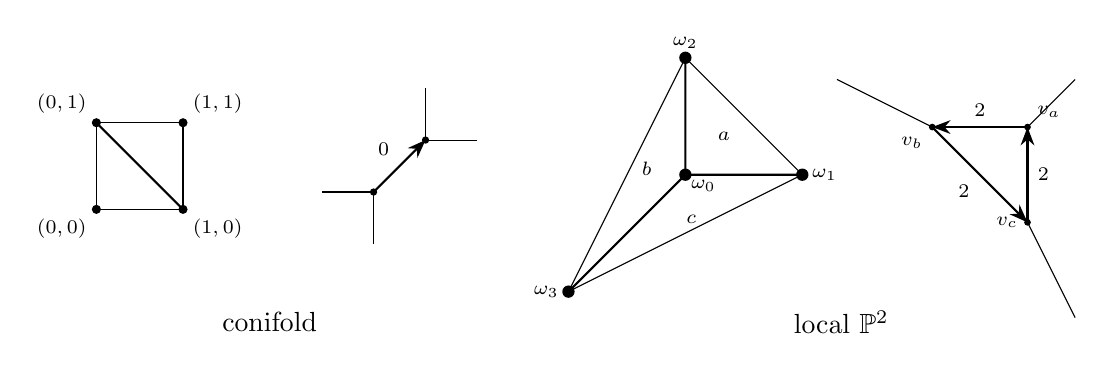
\begin{tikzpicture}[scale=1.1,>=Stealth]
% conifold polygon
\begin{scope}
 \draw (0,0)--(1,0)--(1,1)--(0,1)--cycle; \draw[thick] (1,0)--(0,1);
 \foreach \p in {(0,0),(1,0),(0,1),(1,1)} \fill \p circle (1.5pt);
 \node[below left] at (0,0) {\scriptsize $(0,0)$}; \node[below right] at (1,0) {\scriptsize $(1,0)$};
 \node[above left] at (0,1) {\scriptsize $(0,1)$}; \node[above right] at (1,1) {\scriptsize $(1,1)$};
\end{scope}
\begin{scope}[xshift=3.2cm,yshift=0.2cm,scale=0.6]
 \coordinate (A) at (0,0); \coordinate (B) at (1,1);
 \draw[thick,->] (A)--(B) node[midway,above left] {\scriptsize $0$};
 \draw (A)--++(0,-1) (A)--++(-1,0) (B)--++(1,0) (B)--++(0,1);
 \fill (A) circle (2pt); \fill (B) circle (2pt);
\end{scope}
\node at (2,-1.3) {conifold};
% P2 polygon
\begin{scope}[xshift=6.8cm,yshift=0.4cm,scale=1.35]
 \draw (1,0)--(0,1)--(-1,-1)--cycle; \draw[thick] (0,0)--(1,0) (0,0)--(0,1) (0,0)--(-1,-1);
 \foreach \p in {(0,0),(1,0),(0,1),(-1,-1)} \fill \p circle (1.5pt);
 \node[right] at (1,0) {\scriptsize $\omega_1$}; \node[above] at (0,1) {\scriptsize $\omega_2$};
 \node[left] at (-1,-1) {\scriptsize $\omega_3$}; \node[anchor=north west,inner sep=1pt] at (0.02,-0.02) {\scriptsize $\omega_0$};
 \node at (0.33,0.33) {\scriptsize $a$}; \node at (-0.33,0.05) {\scriptsize $b$}; \node at (0.05,-0.38) {\scriptsize $c$};
\end{scope}
\begin{scope}[xshift=10.2cm,yshift=0.4cm,scale=0.55]
 \coordinate (a) at (1,1); \coordinate (b) at (-1,1); \coordinate (c) at (1,-1);
 \draw[thick,->] (c)--(a) node[midway,right] {\scriptsize $2$};
 \draw[thick,->] (a)--(b) node[midway,above] {\scriptsize $2$};
 \draw[thick,->] (b)--(c) node[midway,below left] {\scriptsize $2$};
 \draw (a)--++(1,1) (b)--++(-2,1) (c)--++(1,-2);
 \foreach \p in {a,b,c} \fill (\p) circle (2pt);
 \node[above right] at (a) {\scriptsize $v_a$}; \node[below left] at (b) {\scriptsize $v_b$}; \node[left] at (c) {\scriptsize $v_c$};
\end{scope}
\node at (8.6,-1.3) {local $\PP^2$};
\end{tikzpicture}

\bigskip
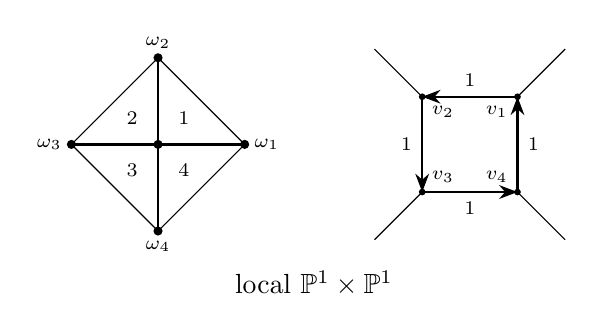
\begin{tikzpicture}[scale=1.1,>=Stealth]
\begin{scope}
 \draw (1,0)--(0,1)--(-1,0)--(0,-1)--cycle; \draw[thick] (1,0)--(-1,0) (0,1)--(0,-1);
 \foreach \p in {(0,0),(1,0),(0,1),(-1,0),(0,-1)} \fill \p circle (1.5pt);
 \node[right] at (1,0) {\scriptsize $\omega_1$}; \node[above] at (0,1) {\scriptsize $\omega_2$};
 \node[left] at (-1,0) {\scriptsize $\omega_3$}; \node[below] at (0,-1) {\scriptsize $\omega_4$};
 \node at (0.3,0.3) {\scriptsize $1$}; \node at (-0.3,0.3) {\scriptsize $2$};
 \node at (-0.3,-0.3) {\scriptsize $3$}; \node at (0.3,-0.3) {\scriptsize $4$};
\end{scope}
\begin{scope}[xshift=3.6cm,scale=0.55]
 \coordinate (v1) at (1,1); \coordinate (v2) at (-1,1); \coordinate (v3) at (-1,-1); \coordinate (v4) at (1,-1);
 \draw[thick,->] (v4)--(v1) node[midway,right] {\scriptsize $1$};
 \draw[thick,->] (v1)--(v2) node[midway,above] {\scriptsize $1$};
 \draw[thick,->] (v2)--(v3) node[midway,left] {\scriptsize $1$};
 \draw[thick,->] (v3)--(v4) node[midway,below] {\scriptsize $1$};
 \draw (v1)--++(1,1) (v2)--++(-1,1) (v3)--++(-1,-1) (v4)--++(1,-1);
 \foreach \p in {v1,v2,v3,v4} \fill (\p) circle (2pt);
 \node[below left] at (v1) {\scriptsize $v_1$}; \node[below right] at (v2) {\scriptsize $v_2$};
 \node[above right] at (v3) {\scriptsize $v_3$}; \node[above left] at (v4) {\scriptsize $v_4$};
\end{scope}
\node at (1.8,-1.6) {local $\PP^1\times\PP^1$};
\end{tikzpicture}
\caption{The three basic examples: triangulated polygon (left) and dual web (right). Interior
segments are drawn thick. In the webs, the arrows are the chosen directions of the internal
edges and the numbers are their framings $n_e$ (Section~\ref{sec:gluing}). The external legs
point in the directions of their $(p,q)$-vectors.}
\label{fig:webs}
\end{figure}

\begin{example}[The webs of Figure~\ref{fig:webs}]\label{ex:webs}
\textit{Local $\PP^2$.} Label the points $\omega_0=(0,0)$, $\omega_1=(1,0)$, $\omega_2=(0,1)$,
$\omega_3=(-1,-1)$ and the triangles $a=\{\omega_0,\omega_1,\omega_2\}$,
$b=\{\omega_0,\omega_2,\omega_3\}$, $c=\{\omega_0,\omega_3,\omega_1\}$ (each listed ccw). The
legs at $v_a$, in ccw order, are $(0,-1)$ (across $\omega_0\omega_1$), $(1,1)$ (external, across
$\omega_1\omega_2$), $(-1,0)$ (across $\omega_2\omega_0$). At $v_b$: $(1,0)$ (across
$\omega_0\omega_2$), $(-2,1)$ (external), $(1,-1)$ (across $\omega_3\omega_0$). At $v_c$:
$(-1,1)$ (across $\omega_0\omega_3$), $(1,-2)$ (external), $(0,1)$ (across $\omega_1\omega_0$).
Placing $v_a=(1,1)$, $v_b=(-1,1)$, $v_c=(1,-1)$ makes all internal edges point along these
vectors.

\textit{Local $\PP^1\times\PP^1$.} With $\omega_1,\ldots,\omega_4=(1,0),(0,1),(-1,0),(0,-1)$ and
triangles $k=\{\omega_0,\omega_k,\omega_{k+1}\}$ ($k$ mod 4), the web is a square with nodes
$v_1=(1,1)$, $v_2=(-1,1)$, $v_3=(-1,-1)$, $v_4=(1,-1)$ and external legs in the diagonal
directions.
\end{example}

\begin{remark}[A compact notation for polygons]\label{rem:corners}
In the package a polygon is specified by the list of its corners, written as \texttt{p=}
followed by the corners \texttt{a,b} separated by underscores. For example
\begin{center}
\begin{tabular}{ll}
\texttt{p=0,0\_1,0\_1,1\_0,1} & (conifold),\\
\texttt{p=1,0\_0,1\_-1,-1} & (local $\PP^2$),\\
\texttt{p=1,0\_0,1\_-1,0\_0,-1} & (local $\PP^1\times\PP^1$).
\end{tabular}
\end{center}
Only the corners are listed. All the other lattice points of the polygon (interior points and
boundary points between corners) are implied. Such a string is read by
\texttt{topvertex.polygon.parse\_polygon}.
\end{remark}

\subsection{Interior versus exterior}

Only interior segments carry information in the partition function: each interior segment
$\tau$ (equivalently, each internal edge $e_\tau$) receives a formal variable $Q_\tau$ and, later,
a partition $\lambda_\tau$ that is summed over. External legs carry nothing (formally, they carry
the empty partition). Therefore the conifold has one variable, local $\PP^2$ three and local
$\PP^1\times\PP^1$ four. (In Section~\ref{sec:classes} we will see that for local $\PP^2$ the
three variables must be set equal, and for $\PP^1\times\PP^1$ they must be set equal in pairs.)

\begin{physrem}
The polygon is the slice of the \textit{fan} of the toric variety $X$ at the level one: the
lattice points $\omega=(a,b)$ give the rays $\hatw=(a,b,1)$, and the triangles give the
3-dimensional cones, i.e.\ the copies of $\C^3$. The fact that all the rays have the third
coordinate equal to $1$ is the Calabi-Yau condition. Unimodularity is smoothness. The web is the
image of the 1-dimensional orbits
of the torus action under a moment map: internal edges are compact curves $\PP^1$, external
legs are non-compact curves $\C$, and interior lattice points are compact divisors (for
local $\PP^2$, the center is the surface $\PP^2$ itself).
\end{physrem}

%=====================================================================================
\subsection{Heights and regular triangulations}\label{ssec:heights}

The last piece of data that we attach to a triangulation is a set of \textit{heights}. The
heights do not enter the formula for $Z$. Their role is to measure the size of a term of $Z$,
which is needed in order to truncate the series consistently (Section~\ref{sec:classes}).

\begin{definition}[Heights, regular triangulation]\label{def:heights}
Let $\omega_1,\ldots,\omega_N$ be the lattice points of $P$. A \textit{height function} $h$
assigns an integer $h_i=h(\omega_i)$, the \textit{height} of $\omega_i$, to every lattice
point. Lift the lattice points to the points $(\omega_i,h_i)\in\R^3$ and take the convex hull of
the lifted points. The faces of the convex hull that are visible from below project to a
subdivision of $P$ into lattice polygons. A triangulation of $P$ is \textit{regular} if it is
the subdivision produced in this way by some height function $h$. In this case
$h_1,\ldots,h_N$ are called \textit{heights of the triangulation}.
\end{definition}

Equivalently, let $\phi_h$ be the continuous function on $P$ that is affine on each triangle
and equal to $h_i$ at $\omega_i$. Then $h_1,\ldots,h_N$ are heights of the triangulation if and
only if $\phi_h$ is strictly convex across every interior segment $\tau$. That is, for the two
triangles $\sigma$ and $\sigma'$ that contain $\tau$, the lifted corner of $\sigma'$ opposite to
$\tau$ lies strictly above the plane through the lifted triangle $\sigma$. The vertical distance
between this corner and the plane is a positive integer $w_\tau$, which we call the
\textit{weight} of $\tau$. An explicit formula for $w_\tau$ is given in (\ref{eq:weights}).

\begin{example}\label{ex:heights}
For the conifold take the height $1$ at $(1,1)$ and $0$ at the other three points. The lower
faces of the lifted tetrahedron are the two triangles of Example~\ref{ex:three}, and the weight
of the diagonal is $1$. The heights $1$ at $(1,0)$, $(0,1)$ and $0$ at $(0,0)$, $(1,1)$ produce
the other triangulation of the square, with the diagonal from $(0,0)$ to $(1,1)$. For local
$\PP^2$ and local $\PP^1\times\PP^1$ one can take the height $0$ at the center and $1$ at the
boundary points. The weights of the interior segments are then $3$ and $2$ respectively.
\end{example}

Heights of a given triangulation are not unique. For example, adding to $h$ an affine function
of the coordinates of the lattice points changes neither the triangulation nor the weights. In
general, different heights give different weights, and therefore different truncations of the
same series $Z$. The heights also provide a way to draw the dual graph. Namely, if the node
$v_\sigma$ is placed at the gradient of $\phi_h$ on $\sigma$, then the internal edge $e_\tau$, drawn
from $v_\sigma$ to $v_{\sigma'}$, is $w_\tau$ times the $(p,q)$-vector (\ref{eq:pq}) of the
corresponding leg at $v_\sigma$. In other words, the weights are the lattice lengths of the
internal edges of the web.

All the triangulations that appear in these notes are regular. Non-regular unimodular
triangulations exist only for larger polygons~\cite{DLRS}. The package finds heights by linear
programming (\texttt{topvertex.polygon.heights}). They can also be supplied by the user, one
integer for each lattice point (the option \texttt{--heights} of the command line).

%=====================================================================================
\section{Partitions and \texorpdfstring{$q$}{q}-numbers}\label{sec:partitions}
%=====================================================================================

In this section we review partitions and $q$-numbers and fix the notation for them.


\subsection{Partitions and Young diagrams}

\begin{definition}
A \textit{partition} is a finite weakly decreasing sequence of positive integers
$\lambda=(\lambda_1\ge\lambda_2\ge\ldots\ge\lambda_\ell>0)$. The $\lambda_i$ are its \textit{parts},
$\ell=\ell(\lambda)$ its \textit{length}, $|\lambda|=\sum_i\lambda_i$ its \textit{size}. If
$|\lambda|=d$ we write $\lambda\vdash d$. The \textit{empty partition} $\es=()$ has size $0$. It is
convenient to set $\lambda_i=0$ for $i>\ell(\lambda)$.
\end{definition}

The \textit{Young diagram} of $\lambda$ is the set of \textit{boxes} $(i,j)\in\Z^2$ with
$1\le i\le\ell(\lambda)$ and $1\le j\le\lambda_i$. We draw row $i$ (with $\lambda_i$ boxes) below
row $i-1$, all rows left-justified. For example $(3,1)$ is \yd{3,1}\,, and $(2,2,1)$ is
\yd{2,2,1}\,. We identify a partition with its diagram and write $s\in\lambda$ for a box.

\begin{definition}
The \textit{conjugate} (or transposed) partition $\lt\lambda$ has the transposed diagram: its
$j$-th part is the length of the $j$-th column of $\lambda$,
$\lt\lambda_j=\#\{i:\lambda_i\ge j\}$. For example $\lt{(3,1)}=(2,1,1)$. Note that
$(\lt\lambda)^{\tr}=\lambda$ and $|\lt\lambda|=|\lambda|$.
\end{definition}

\begin{definition}
The \textit{content} of the box $s=(i,j)$ is $c(s)=j-i$ (constant along diagonals). For a partition
$\lambda$ put
\begin{equation}\label{eq:kappa}
\kappa(\lambda)=\sum_{i\ge1}\lambda_i(\lambda_i-2i+1).
\end{equation}
\end{definition}

\begin{lemma}\label{lem:kappa}
$\kappa(\lambda)=2\sum_{s\in\lambda}c(s)$. Consequently $\kappa(\lambda)$ is even and
$\kappa(\lt\lambda)=-\kappa(\lambda)$.
\end{lemma}
\begin{proof}
The contents in row $i$ are $1-i,2-i,\ldots,\lambda_i-i$, with sum
$\lambda_i(\lambda_i+1)/2-i\lambda_i=\lambda_i(\lambda_i-2i+1)/2$. Summing over $i$ gives the
formula, and therefore evenness. Transposing exchanges $i$ and $j$, so every content changes sign.
\end{proof}

For example, the contents of $(3,1)$ are $0,1,2$ in the first row and $-1$ in the second, so
$\kappa(3,1)=2(0+1+2-1)=4$. Directly from the definition (\ref{eq:kappa}) one gets
$3\cdot 2+1\cdot(-2)=4$.

\begin{physrem}
The quadratic Casimir of the representation of $U(N)$ with the highest weight $\lambda$ is
$\sum_i\lambda_i(\lambda_i-2i+1+N)=\kappa(\lambda)+N|\lambda|$, in the normalization in which
the fundamental representation has the Casimir $N$. This is how $\kappa$ enters the topological
vertex: in Chern-Simons theory, changing the framing of a knot multiplies the Wilson loop in the
representation $\lambda$ by a phase governed by the quadratic Casimir.
\end{physrem}

\begin{definition}
For a box $s=(i,j)\in\lambda$, the \textit{arm} $a(s)=\lambda_i-j$ is the number of boxes to its
right, the \textit{leg} $l(s)=\lt\lambda_j-i$ the number of boxes below it, and the \textit{hook
length} is $h(s)=a(s)+l(s)+1$.
\end{definition}

For $(3,1)$ the hook lengths are $4,2,1$ in the first row and $1$ in the second. Transposition
exchanges arms and legs, so $\lambda$ and $\lt\lambda$ have the same multiset of hook lengths.
Table~\ref{tab:partitions} lists everything for $|\lambda|\le 4$.

\begin{table}[ht]
\centering
\begin{tabular}{cccccc}
\toprule
$\lambda$ & diagram & $\lt\lambda$ & contents (row by row) & $\kappa(\lambda)$ & hook lengths\\
\midrule
$(1)$ & \yd{1} & $(1)$ & $0$ & $0$ & $1$\\[2pt]
$(2)$ & \yd{2} & $(1,1)$ & $0,1$ & $2$ & $2,1$\\
$(1,1)$ & \yd{1,1} & $(2)$ & $0\,|\,{-1}$ & $-2$ & $2\,|\,1$\\[2pt]
$(3)$ & \yd{3} & $(1,1,1)$ & $0,1,2$ & $6$ & $3,2,1$\\
$(2,1)$ & \yd{2,1} & $(2,1)$ & $0,1\,|\,{-1}$ & $0$ & $3,1\,|\,1$\\
$(1,1,1)$ & \yd{1,1,1} & $(3)$ & $0\,|\,{-1}\,|\,{-2}$ & $-6$ & $3\,|\,2\,|\,1$\\[2pt]
$(4)$ & \yd{4} & $(1,1,1,1)$ & $0,1,2,3$ & $12$ & $4,3,2,1$\\
$(3,1)$ & \yd{3,1} & $(2,1,1)$ & $0,1,2\,|\,{-1}$ & $4$ & $4,2,1\,|\,1$\\
$(2,2)$ & \yd{2,2} & $(2,2)$ & $0,1\,|\,{-1},0$ & $0$ & $3,2\,|\,2,1$\\
$(2,1,1)$ & \yd{2,1,1} & $(3,1)$ & $0,1\,|\,{-1}\,|\,{-2}$ & $-4$ & $4,1\,|\,2\,|\,1$\\
$(1,1,1,1)$ & \yd{1,1,1,1} & $(4)$ & $0\,|\,{-1}\,|\,{-2}\,|\,{-3}$ & $-12$ & $4\,|\,3\,|\,2\,|\,1$\\
\bottomrule
\end{tabular}
\caption{All partitions of size $1\le|\lambda|\le4$. Rows of the diagram are separated by
``$|$''.}
\label{tab:partitions}
\end{table}

\subsection{\texorpdfstring{$q$}{q}-numbers}

As a reminder, $x=q^{1/2}$. All our functions will be rational functions of $x$, and a power
$q^{k/2}$ means
$x^k$.

\begin{definition}
For an integer $k$, the \textit{$q$-number} is
\begin{equation}\label{eq:qnumber}
[k]=q^{k/2}-q^{-k/2}=x^k-x^{-k}.
\end{equation}
\end{definition}

\begin{lemma}\label{lem:qnumbers}
\begin{enumerate}
\item $[0]=0$, $[-k]=-[k]$, and $[k]$ is odd under $q\rightarrow1/q$ (i.e.\ $x\rightarrow1/x$).
\item $[k]^2=q^k-2+q^{-k}$, in particular $[1]^2=q-2+q^{-1}$.
\item For $k\ge1$, $[k]=[1]\,(q^{(k-1)/2}+q^{(k-3)/2}+\ldots+q^{-(k-1)/2})$ ($k$ terms). In
particular $[2]=[1](q^{1/2}+q^{-1/2})$ and $[3]=[1](q+1+q^{-1})$.
\item $1-q^{-k}=q^{-k/2}[k]$ and $q^k-1=q^{k/2}[k]$.
\end{enumerate}
\end{lemma}
\begin{proof}
Direct computation. For (3) multiply out (a telescoping sum).
\end{proof}

Throughout the notes we use the abbreviation
\begin{equation}\label{eq:y}
y:=[1]^2=q-2+q^{-1}.
\end{equation}
Many symmetric expressions are polynomials in $y$:
\begin{multline}
q+q^{-1}=y+2,\qquad q-1+q^{-1}=y+1,\qquad q^2+q^{-2}=y^2+4y+2,\\
[2]^2=y(y+4),\qquad [3]^2=y(y+3)^2 .
\end{multline}
(For instance $[2]^2=[1]^2(q^{1/2}+q^{-1/2})^2=y(q+2+q^{-1})=y(y+4)$.) Since $y$ itself is
invariant under $q\rightarrow 1/q$, so is every polynomial in $y$. Conversely, every Laurent polynomial in
$q$ invariant under $q\rightarrow1/q$ is a polynomial in $y$ (Exercise~\ref{ex:ypoly}).

\begin{exercise}\label{ex:part1}
For $\lambda=(3,2)$ find $\lt\lambda$, the contents, $\kappa(\lambda)$ (in two ways) and the hook
lengths. Check that $5!/\prod_s h(s)=5$.
\end{exercise}

\begin{exercise}\label{ex:part2}
Show that $\kappa(\lambda)=\sum_i\lambda_i^2-\sum_j(\lt\lambda_j)^2$, which gives another proof
of $\kappa(\lt\lambda)=-\kappa(\lambda)$.
\end{exercise}

\begin{exercise}\label{ex:ypoly}
(a) Express $q^3+q^{-3}$ as a polynomial in $y$. (b) Show by induction on the top power that
every Laurent polynomial $P(q)$ with $P(q)=P(1/q)$ is a polynomial in $y$, and that the
coefficient of the top power $y^G$ equals the coefficient of $q^G$ in $P$.
\end{exercise}

%=====================================================================================
\section{Schur functions, concretely}\label{sec:schur}
%=====================================================================================

In this section we define Schur and skew Schur functions by explicit determinants, and
evaluate them at the specializations that enter the vertex. Since the letter $x$ is reserved for
$q^{1/2}$, a sequence of variables will be denoted $\vu=(u_1,u_2,u_3,\ldots)$. It may be finite
or infinite.

\subsection{Elementary and complete symmetric functions}

\begin{definition}
The \textit{elementary} and \textit{complete} symmetric functions $e_k(\vu)$, $h_k(\vu)$
($k\ge0$) are defined by the generating functions
\begin{equation}\label{eq:EH}
E_\vu(z)=\sum_{k\ge0}e_k(\vu)z^k=\prod_{i\ge1}(1+u_iz),\qquad
H_\vu(z)=\sum_{k\ge0}h_k(\vu)z^k=\prod_{i\ge1}\frac1{1-u_iz}.
\end{equation}
We also set $e_k=h_k=0$ for $k<0$.
\end{definition}

In particular, $e_0=h_0=1$, $e_1=h_1=\sum_iu_i$, $e_2=\sum_{i<j}u_iu_j$ and $h_2=\sum_{i\le j}u_iu_j$. In
general, $e_k$ is the sum of all products of $k$ \textit{distinct} variables and $h_k$ the sum of
all monomials of degree $k$. Since $E_\vu(-z)H_\vu(z)=1$,
\begin{equation}\label{eq:EHrel}
\sum_{j=0}^k(-1)^je_j(\vu)h_{k-j}(\vu)=0\qquad(k\ge1).
\end{equation}

\begin{remark}[Infinite sequences]
We will only use two kinds of infinite sequences, $u_i=q^{-i+1/2}$ and the same sequence with
finitely many terms changed. For these, think of $q^{-1/2}$ as a small number (or as a formal
variable): then all the infinite sums and products above converge (as power series in $q^{-1/2}$)
and, as we show below, they are \textit{rational functions} of $x=q^{1/2}$. From then on we only
work with these rational functions, and forget the expansion.
\end{remark}

\subsection{Skew Schur functions by Jacobi-Trudi}

\begin{definition}[Jacobi-Trudi]\label{def:JT}
For partitions $\mu,\nu$ the \textit{skew Schur function} is the determinant
\begin{equation}\label{eq:JT}
s_{\mu/\nu}(\vu)=\det\big(h_{\mu_i-\nu_j-i+j}(\vu)\big)_{1\le i,j\le\ell(\mu)}
=\det\big(e_{\lt\mu_i-\lt\nu_j-i+j}(\vu)\big)_{1\le i,j\le\ell(\lt\mu)} .
\end{equation}
For $\nu=\es$ we write $s_\mu=s_{\mu/\es}$ (the \textit{Schur function}), and $s_\es=1$.
\end{definition}

The equality of the two determinants is a classical theorem~\cite[I.(5.5)]{Macdonald}. One
can take either as the definition, and check the equality in examples. Two facts that follow
from the definition (\cite[I.5]{Macdonald}): $s_{\mu/\nu}=0$ unless $\nu\subset\mu$ (the diagram
of $\nu$ is contained in that of $\mu$), and $s_{\mu/\mu}=1$. In particular, in all our sums over
$\eta$ only $\eta\subset\mu$ contributes, so the sums are finite.

\begin{example}\label{ex:smallschur}
\begin{align}
s_{(1)}&=h_1=e_1,\qquad s_{(2)}=h_2,\qquad
s_{(1,1)}=\det\begin{pmatrix}h_1&h_2\\h_0&h_1\end{pmatrix}=h_1^2-h_2=e_2,\\
s_{(2,1)}&=\det\begin{pmatrix}h_2&h_3\\h_0&h_1\end{pmatrix}=h_1h_2-h_3,\qquad
s_{(2,1)/(1)}=\det\begin{pmatrix}h_1&h_3\\0&h_1\end{pmatrix}=h_1^2,\\
s_{(2)/(1)}&=h_1,\qquad s_{(1)/(1)}=h_0=1 .
\end{align}
For $s_{(1,1)}$ the $e$-form gives directly $e_2$ (since $\lt{(1,1)}=(2)$), and $h_1^2-h_2=e_2$
is (\ref{eq:EHrel}) for $k=2$. For $s_{(2,1)/(1)}$: $\mu=(2,1)$, $\nu=(1,0)$, and the entries are
$h_{2-1-1+1}=h_1$, $h_{2-0-1+2}=h_3$, $h_{1-1-2+1}=h_{-1}=0$, $h_{1-0-2+2}=h_1$.
\end{example}

\subsection{The specialization \texorpdfstring{$q^\rho$}{q\textasciicircum rho}}

\begin{definition}
$\qrho$ denotes the infinite sequence $u_i=q^{-i+1/2}$, i.e.\
$\qrho=(q^{-1/2},q^{-3/2},q^{-5/2},\ldots)$. For a symmetric function $f$ we write $f(\qrho)$ for
its value at this sequence.
\end{definition}

\begin{proposition}\label{prop:hrho}
\begin{equation}\label{eq:hrho}
h_k(\qrho)=\frac{q^{k(k-1)/4}}{[1][2]\cdots[k]},\qquad
e_k(\qrho)=\frac{q^{-k(k-1)/4}}{[1][2]\cdots[k]}\qquad(k\ge0).
\end{equation}
\end{proposition}
\begin{proof}
Put $a=q^{-1}$ and $w=q^{-1/2}z$, so that $u_iz=a^{i-1}w$. Then
$E(z)=f(w):=\prod_{i\ge0}(1+a^iw)$ satisfies $f(w)=(1+w)f(aw)$. Writing
$f(w)=\sum_kc_kw^k$ and comparing coefficients of $w^k$ gives $c_k=a^kc_k+a^{k-1}c_{k-1}$, i.e.\
$c_k=\frac{a^{k-1}}{1-a^k}c_{k-1}$, $c_0=1$, so that
\begin{equation}
\prod_{i\ge0}(1+a^iw)=\sum_{k\ge0}\frac{a^{k(k-1)/2}}{(1-a)(1-a^2)\cdots(1-a^k)}\,w^k .
\end{equation}
Similarly $g(w)=\prod_{i\ge0}(1-a^iw)^{-1}$ satisfies $(1-w)g(w)=g(aw)$, which gives
$c_k=c_{k-1}/(1-a^k)$ and $g(w)=\sum_kw^k/((1-a)\cdots(1-a^k))$. Now substitute back, using
$1-q^{-j}=q^{-j/2}[j]$ (Lemma~\ref{lem:qnumbers}), so that $\prod_{j=1}^k(1-q^{-j})=
q^{-k(k+1)/4}[1]\cdots[k]$:
\begin{multline}
h_k(\qrho)=\frac{q^{-k/2}}{\prod_{j\le k}(1-q^{-j})}=\frac{q^{-k/2+k(k+1)/4}}{[1]\cdots[k]},\\
e_k(\qrho)=\frac{q^{-k/2}q^{-k(k-1)/2}}{\prod_{j\le k}(1-q^{-j})}
=\frac{q^{-k/2-k(k-1)/2+k(k+1)/4}}{[1]\cdots[k]},
\end{multline}
and the exponents simplify to $k(k-1)/4$ and $-k(k-1)/4$.
\end{proof}

For instance $h_1(\qrho)=e_1(\qrho)=1/[1]$ (which is just the geometric series
$\sum_iq^{-i+1/2}=q^{-1/2}/(1-q^{-1})$), $h_2(\qrho)=q^{1/2}/([1][2])$,
$e_2(\qrho)=q^{-1/2}/([1][2])$, $h_3(\qrho)=q^{3/2}/([1][2][3])$.

\begin{theorem}[Hook formula]\label{thm:hook}
\begin{equation}\label{eq:hook}
s_\lambda(\qrho)=\frac{q^{\kappa(\lambda)/4}}{\prod_{s\in\lambda}[h(s)]} .
\end{equation}
Consequently $s_{\lt\lambda}(\qrho)=q^{-\kappa(\lambda)/2}s_\lambda(\qrho)$ and
$s_\lambda(\qrho)\,s_{\lt\lambda}(\qrho)=\prod_{s\in\lambda}[h(s)]^{-2}$.
\end{theorem}

This is \cite[I.3, Ex.~2]{Macdonald} rewritten with $q$-numbers. We do not prove it, but check
it in the four smallest cases, using Example~\ref{ex:smallschur}, (\ref{eq:hrho}) and
Table~\ref{tab:partitions}:
\begin{itemize}
\item $\lambda=(1)$: $s_{(1)}(\qrho)=h_1(\qrho)=1/[1]$, hook formula: $q^0/[1]$. \checkmark
\item $\lambda=(2)$: $h_2(\qrho)=q^{1/2}/([1][2])$, hook formula: $q^{2/4}/([2][1])$. \checkmark
\item $\lambda=(1,1)$: $e_2(\qrho)=q^{-1/2}/([1][2])$, hook formula: $q^{-2/4}/([2][1])$. \checkmark
\item $\lambda=(2,1)$: $h_1h_2-h_3=\frac{q^{1/2}}{[1]^2[2]}-\frac{q^{3/2}}{[1][2][3]}
=\frac{q^{1/2}[3]-q^{3/2}[1]}{[1]^2[2][3]}=\frac{q-q^{-1}}{[1]^2[2][3]}=\frac{1}{[1]^2[3]}$,
since $q^{1/2}[3]-q^{3/2}[1]=(q^2-q^{-1})-(q^2-q)=q-q^{-1}=[2]$. Hook formula: hooks $3,1,1$
and $\kappa=0$. \checkmark
\end{itemize}
The two consequences follow because $\lambda$ and $\lt\lambda$ have the same hook lengths and
$\kappa(\lt\lambda)=-\kappa(\lambda)$.

\subsection{The specialization \texorpdfstring{$q^{\nu+\rho}$}{q\textasciicircum(nu+rho)}}

\begin{definition}
For a partition $\nu$, $\qlr{\nu}$ denotes the sequence $u_i=q^{\nu_i-i+1/2}$, $i\ge1$ (recall
$\nu_i=0$ for $i>\ell(\nu)$). It differs from $\qrho$ only in the first $\ell(\nu)$ terms.
\end{definition}

\begin{proposition}[{\cite[(3)]{Kon}}]\label{prop:hnu}
\begin{align}
\sum_{k\ge0}h_k(\qlr\nu)z^k&=\prod_{i=1}^{\ell(\nu)}\frac{1-q^{-i+1/2}z}{1-q^{\nu_i-i+1/2}z}
\cdot\sum_{k\ge0}h_k(\qrho)z^k,\label{eq:hnu}\\
\sum_{k\ge0}e_k(\qlr\nu)z^k&=\prod_{i=1}^{\ell(\nu)}\frac{1+q^{\nu_i-i+1/2}z}{1+q^{-i+1/2}z}
\cdot\sum_{k\ge0}e_k(\qrho)z^k.\label{eq:enu}
\end{align}
\end{proposition}
\begin{proof}
In the product $H_{\qlr\nu}(z)=\prod_i(1-u_iz)^{-1}$ replace the first $\ell(\nu)$ factors by
those of $\qrho$, multiplying and dividing by the old ones. Same for $E$.
\end{proof}

The prefactor in (\ref{eq:hnu}) is a \textit{finite} rational function of $z$, so $h_k(\qlr\nu)$ is
obtained by expanding it as a power series in $z$ (only the coefficients up to $z^k$ are
needed) and multiplying by the known series $\sum h_k(\qrho)z^k$. This, together with
Jacobi-Trudi, computes every $s_{\mu/\eta}(\qlr\nu)$ in finitely many steps.

\begin{example}[$\nu=(1)$]\label{ex:h1nu}
Here $\qlr{(1)}=(q^{1/2},q^{-3/2},q^{-5/2},\ldots)$ and the prefactor is
$\frac{1-az}{1-bz}$ with $a=q^{-1/2}$, $b=q^{1/2}$. Expanding,
$\frac{1-az}{1-bz}=1+(b-a)z+(b-a)bz^2+\ldots$ and $b-a=[1]$. Therefore
\begin{align}
h_1(\qlr{(1)})&=h_1(\qrho)+[1]=\frac1{[1]}+[1]=\frac{1+[1]^2}{[1]}=\frac{q-1+q^{-1}}{[1]}=\frac{y+1}{[1]},\\
h_2(\qlr{(1)})&=h_2(\qrho)+[1]h_1(\qrho)+[1]q^{1/2}=\frac{q^{1/2}}{[1][2]}+1+q^{1/2}[1]
=q+\frac{q^{1/2}}{[1][2]} .
\end{align}
(Check of the first line: $\sum_iu_i=q^{1/2}+\sum_{i\ge2}q^{-i+1/2}=q^{1/2}+q^{-1}/[1]$, and
$q^{1/2}[1]+q^{-1}=q-1+q^{-1}$.) Consequently, from Example~\ref{ex:smallschur},
\begin{multline}
s_{(1)}(\qlr{(1)})=s_{(2)/(1)}(\qlr{(1)})=h_1(\qlr{(1)})=\frac{y+1}{[1]},\\
s_{(1)/(1)}(\qlr{(1)})=1,\qquad s_{(2)}(\qlr{(1)})=q+\frac{q^{1/2}}{[1][2]} .
\end{multline}
\end{example}

\begin{exercise}\label{ex:schur1}
Compute $s_{(3)}(\qrho)$ and $s_{(1,1,1)}(\qrho)$ from (\ref{eq:hrho}) and compare with the
hook formula.
\end{exercise}

\begin{exercise}\label{ex:schur2}
Use (\ref{eq:enu}) to show $e_1(\qlr{(1)})=h_1(\qlr{(1)})$ and
$s_{(1,1)}(\qlr{(1)})=e_2(\qlr{(1)})=q^{-1}+\frac{q^{-1/2}}{[1][2]}$.
\end{exercise}

\begin{exercise}\label{ex:schur3}
Check the two forms of Jacobi-Trudi (\ref{eq:JT}) against each other for $\mu=(2,1)$, $\nu=\es$,
using (\ref{eq:EHrel}).
\end{exercise}

%=====================================================================================
\section{The vertex \texorpdfstring{$C_{\lambda_1\lambda_2\lambda_3}(q)$}{C(q)}}\label{sec:vertex}
%=====================================================================================

In this section we define the vertex, describe its symmetries and special cases, and list its
values for small partitions.

\subsection{Definition and symmetries}

\begin{definition}[Topological vertex {\cite[Def.~2.2]{Kon}}]\label{def:vertex}
For three partitions $\lambda_1,\lambda_2,\lambda_3$,
\begin{equation}\label{eq:vertex}
C_{\lambda_1\lambda_2\lambda_3}(q)=q^{\kappa(\lambda_3)/2}\,s_{\lambda_2}(\qrho)
\sum_{\eta}s_{\lambda_1/\eta}\big(q^{\lt\lambda_2+\rho}\big)\,
s_{\lt\lambda_3/\eta}\big(q^{\lambda_2+\rho}\big).
\end{equation}
The sum runs over all partitions $\eta$, but only $\eta\subset\lambda_1$ and $\eta\subset\lt\lambda_3$
contribute, so it is finite. $C$ is a rational function of $x=q^{1/2}$.
\end{definition}

Note where the transposes are: the first skew Schur function is evaluated at $q^{\lt\lambda_2+\rho}$
and has $\lambda_1$ on top, whereas the second is evaluated at $q^{\lambda_2+\rho}$ and has $\lt\lambda_3$
on top.

\begin{theorem}[Cyclic symmetry, {\cite{ORV}}]\label{thm:cyclic}
$C_{\lambda_1\lambda_2\lambda_3}=C_{\lambda_2\lambda_3\lambda_1}=C_{\lambda_3\lambda_1\lambda_2}$.
\end{theorem}

This is not obvious from the definition (\ref{eq:vertex}), in which the three slots play
different roles. It is proved
in~\cite{ORV} by interpreting $C$ as a generating function of plane partitions. We use it freely,
and one can check it on the examples below. It means that only the \textit{cyclic order} of the
three partitions matters. (Exchanging two of them is \textit{not} a symmetry. Instead one has
$C_{\lambda_1\lambda_2\lambda_3}=q^{(\kappa(\lambda_1)+\kappa(\lambda_2)+\kappa(\lambda_3))/2}\,
C_{\lt\lambda_1\lt\lambda_3\lt\lambda_2}$, \cite[(3.12)]{AKMV}, which we will not need, but
which the package verifies, see Exercise~\ref{ex:vertex3}.)

\subsection{Special cases}

Directly from (\ref{eq:vertex}), using $s_{\es}=1$ and $s_{\es/\eta}=0$ for $\eta\ne\es$:
\begin{align}
C_{\lambda\es\es}&=s_\lambda(\qrho),\label{eq:C100}\\
C_{\lambda\mu\es}&=s_\mu(\qrho)\,s_\lambda(q^{\lt\mu+\rho}),\label{eq:C110}\\
C_{\lambda\es\nu}&=q^{\kappa(\nu)/2}\sum_\eta s_{\lambda/\eta}(\qrho)\,s_{\lt\nu/\eta}(\qrho),\label{eq:C101}\\
C_{\es\es\nu}&=q^{\kappa(\nu)/2}s_{\lt\nu}(\qrho)=s_\nu(\qrho)\label{eq:C001}
\end{align}
(the last step by Theorem~\ref{thm:hook}, consistent with cyclic symmetry and (\ref{eq:C100})).

\subsection{Three computations by hand}

\begin{example}[$C_{(1)\es\es}$, $C_{(2)\es\es}$, $C_{(1,1)\es\es}$]
By (\ref{eq:C100}) and the hook formula,
\begin{equation}
C_{(1)\es\es}=\frac1{[1]},\qquad C_{(2)\es\es}=\frac{q^{1/2}}{[1][2]}=\frac{q^2}{(q-1)(q^2-1)},\qquad
C_{(1,1)\es\es}=\frac{q^{-1/2}}{[1][2]}=\frac{q}{(q-1)(q^2-1)},
\end{equation}
using $[1][2]=(q-1)(q^2-1)q^{-3/2}$ (Lemma~\ref{lem:qnumbers}(4)).
\end{example}

\begin{example}[$C_{(1)(1)\es}$]\label{ex:C110}
By (\ref{eq:C110}) with $\lambda=\mu=(1)$, $\lt\mu=(1)$, and Example~\ref{ex:h1nu},
\begin{equation}
C_{(1)(1)\es}=s_{(1)}(\qrho)\,s_{(1)}(\qlr{(1)})=\frac1{[1]}\cdot\frac{y+1}{[1]}=\frac{y+1}{y}
=\frac{q-1+q^{-1}}{q-2+q^{-1}}=\frac{q^2-q+1}{(1-q)^2}.
\end{equation}
By cyclic symmetry this is also $C_{(1)\es(1)}$ and $C_{\es(1)(1)}$. Let us check one of these
directly: by (\ref{eq:C101}), $C_{(1)\es(1)}=q^0\big(s_{(1)}(\qrho)^2+s_{(1)/(1)}(\qrho)^2\big)
=\frac1y+1=\frac{y+1}{y}$, the two terms coming from $\eta=\es$ and $\eta=(1)$. \checkmark
\end{example}

\begin{example}[$C_{(1)(1)(1)}$]\label{ex:C111}
Now $\lambda_1=\lambda_2=\lambda_3=(1)$, $\kappa((1))=0$, and $\eta\in\{\es,(1)\}$:
\begin{equation}
C_{(1)(1)(1)}=s_{(1)}(\qrho)\Big(s_{(1)}(\qlr{(1)})^2+s_{(1)/(1)}(\qlr{(1)})^2\Big)
=\frac1{[1]}\Big(\frac{(y+1)^2}{y}+1\Big)=\frac{y^2+3y+1}{[1]^3}.
\end{equation}
In terms of $q$: $y^2+3y+1=q^2-q+1-q^{-1}+q^{-2}$ and $[1]^3=q^{-3/2}(q-1)^3$, so
\begin{equation}
C_{(1)(1)(1)}=\frac{q^4-q^3+q^2-q+1}{q^{1/2}(q-1)^3}.
\end{equation}
\end{example}

These agree with the values listed in~\cite[p.~6]{Kon}. Table~\ref{tab:vertex} lists all
vertices with $|\lambda_1|+|\lambda_2|+|\lambda_3|\le3$, one representative per cyclic orbit.

\begin{table}[ht]
\centering
\renewcommand{\arraystretch}{1.25}
% GENERATED by notes/make_tables.py from the topvertex package -- do not edit by hand.
\begin{tabular}{ll}
\toprule
$(\lambda_1,\lambda_2,\lambda_3)$ & $C_{\lambda_1\lambda_2\lambda_3}(q)$\\
\midrule
$(\es,\es,\es)$ & $\displaystyle 1$ \\[6pt]
$((1),\es,\es)$ & $\displaystyle \frac{1}{[1]}$ \\[6pt]
$((2),\es,\es)$ & $\displaystyle \frac{q^{1/2}}{[1][2]}$ \\[6pt]
$((1,1),\es,\es)$ & $\displaystyle \frac{q^{-1/2}}{[1][2]}$ \\[6pt]
$((1),(1),\es)$ & $\displaystyle \frac{q - 1 + q^{-1}}{[1]^{2}}$ \\[6pt]
$((3),\es,\es)$ & $\displaystyle \frac{q^{3/2}}{[1][2][3]}$ \\[6pt]
$((2,1),\es,\es)$ & $\displaystyle \frac{1}{[1]^{2}[3]}$ \\[6pt]
$((1,1,1),\es,\es)$ & $\displaystyle \frac{q^{-3/2}}{[1][2][3]}$ \\[6pt]
$((2),(1),\es)$ & $\displaystyle \frac{q^{5/2} - q^{3/2} + q^{-1/2}}{[1]^{2}[2]}$ \\[6pt]
$((1,1),(1),\es)$ & $\displaystyle \frac{q^{1/2} - q^{-3/2} + q^{-5/2}}{[1]^{2}[2]}$ \\[6pt]
$((2),\es,(1))$ & $\displaystyle \frac{q^{3/2} - q^{-1/2} + q^{-3/2}}{[1]^{2}[2]}$ \\[6pt]
$((1,1),\es,(1))$ & $\displaystyle \frac{q^{3/2} - q^{1/2} + q^{-3/2}}{[1]^{2}[2]}$ \\[6pt]
$((1),(1),(1))$ & $\displaystyle \frac{q^{2} - q + 1 - q^{-1} + q^{-2}}{[1]^{3}}$ \\[6pt]
\bottomrule
\end{tabular}

\caption{(Generated.) The vertex $C_{\lambda_1\lambda_2\lambda_3}(q)$ for
$|\lambda_1|+|\lambda_2|+|\lambda_3|\le 3$, in lowest terms, with the denominator written as a
product of $q$-numbers $[k]=q^{k/2}-q^{-k/2}$. One representative of each cyclic orbit is listed,
and the others follow from Theorem~\ref{thm:cyclic}.}
\label{tab:vertex}
\end{table}

\begin{exercise}\label{ex:vertex1}
Compute $C_{(2)(1)\es}=s_{(1)}(\qrho)s_{(2)}(\qlr{(1)})$ with Example~\ref{ex:h1nu} and compare
with Table~\ref{tab:vertex}. Then compute $C_{\es(2)(1)}$ from (\ref{eq:vertex}) directly (one
needs $s_{(1)}(q^{(2)+\rho})$) and confirm cyclic symmetry in this case.
\end{exercise}

\begin{exercise}\label{ex:vertex2}
Show that $C_{\lambda\es\es}(q)$ and $C_{\lt\lambda\es\es}(q)$ are exchanged by $q\rightarrow1/q$ up to
the sign $(-1)^{|\lambda|}$. (In general $C_{\lambda\mu\nu}(1/q)=(-1)^{|\lambda|+|\mu|+|\nu|}
C_{\lt\lambda\lt\mu\lt\nu}(q)$.)
\end{exercise}

\begin{exercise}\label{ex:vertex3}
Verify $C_{(2)\es\es}=q\,C_{(1,1)\es\es}$, a special case of the transposition identity quoted
after Theorem~\ref{thm:cyclic}.
\end{exercise}

%=====================================================================================
\section{Framings and the gluing rule}\label{sec:gluing}
%=====================================================================================

In this section we define the framings of the internal edges of the dual graph and state the
gluing formula for $Z$.


\subsection{The framing of a flag}\label{ssec:framing}

Let $\tau$ be an interior segment with endpoints $\omega_1,\omega_2$, and let
$\sigma=\{\omega_1,\omega_2,\omega_3\}$ and $\sigma'=\{\omega_1,\omega_2,\omega_3'\}$ be the two
triangles containing it. A \textit{flag} is a pair $f=(v_\sigma,e_\tau)$ of a node and an internal
edge ending at it. The same edge seen from the other end is the flag $-f=(v_{\sigma'},e_\tau)$.
We always \textit{name the endpoints of $\tau$ so that $(\omega_1,\omega_2,\omega_3)$ is
counterclockwise}. Then $(\omega_2,\omega_1,\omega_3')$ is counterclockwise as well, because
$\omega_3$ and $\omega_3'$ lie on opposite sides of $\tau$.

\begin{center}
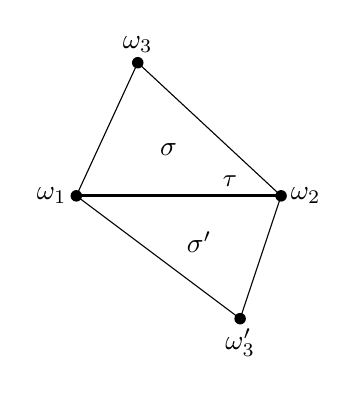
\begin{tikzpicture}[scale=1.3]
 \coordinate (w1) at (0,0); \coordinate (w2) at (2,0); \coordinate (w3) at (0.6,1.3); \coordinate (w3p) at (1.6,-1.2);
 \draw (w1)--(w3)--(w2) (w1)--(w3p)--(w2); \draw[very thick] (w1)--(w2);
 \foreach \p in {w1,w2,w3,w3p} \fill (\p) circle (1.6pt);
 \node[left] at (w1) {$\omega_1$}; \node[right] at (w2) {$\omega_2$};
 \node[above] at (w3) {$\omega_3$}; \node[below] at (w3p) {$\omega_3'$};
 \node at (0.9,0.45) {$\sigma$}; \node at (1.2,-0.45) {$\sigma'$}; \node[above] at (1.5,0) {\small $\tau$};
\end{tikzpicture}
\end{center}

\begin{lemma}\label{lem:a1a2}
There are unique integers $a_1,a_2$ with
\begin{equation}\label{eq:relation}
\hatw_3'=-a_1\hatw_1-a_2\hatw_2-\hatw_3,\qquad\text{and they satisfy}\qquad a_1+a_2=-2 .
\end{equation}
\end{lemma}
\begin{proof}
By Lemma~\ref{lem:unimodular}, $\hatw_1,\hatw_2,\hatw_3$ is a basis of $\Z^3$, so
$\hatw_3'=c_1\hatw_1+c_2\hatw_2+c_3\hatw_3$ with integers $c_i$. Taking the determinant with
$\hatw_1,\hatw_2$ and using (\ref{eq:det3}): $\det(\omega_1,\omega_2,\omega_3')=c_3\det(\omega_1,
\omega_2,\omega_3)$. The left side is $-1$ (the triangle $\sigma'$ is unimodular and
$(\omega_1,\omega_2,\omega_3')$ is clockwise) and the right side is $c_3\cdot1$, so $c_3=-1$.
Comparing third components (all equal to $1$) gives $1=c_1+c_2-1$, i.e.\ $a_1+a_2=-c_1-c_2=-2$.
\end{proof}

\begin{definition}[Framing, {\cite[\S4.2]{Kon}}]\label{def:framing}
With $(\omega_1,\omega_2,\omega_3)$ counterclockwise and $a_1,a_2$ as in (\ref{eq:relation}), the
\textit{framing} of the flag $f=(v_\sigma,e_\tau)$ is
\begin{equation}\label{eq:framing}
n_f=\frac{a_1-a_2}{2}=a_1+1 .
\end{equation}
\end{definition}

In plain language, the framing is an integer attached to each end of an internal edge that
records how the neighborhood of the corresponding curve is twisted. In the formula for $Z$ it
appears only through the factor $q^{n\kappa(\lambda)/2}$ and a sign.

\begin{lemma}\label{lem:framingprops}
\begin{enumerate}
\item $n_{-f}=-n_f$.
\item (Recipe.) $n_f=\det(\omega_1,\omega_3',\omega_3)-1$, with $\det$ as in (\ref{eq:det}).
\item If an affine map $\omega\mapsto A\omega+b$ with $A\in SL(2,\Z)$, $b\in\Z^2$, brings
$\omega_1,\omega_2,\omega_3$ to $(0,0),(1,0),(0,1)$, it brings $\omega_3'$ to $(n_f+1,-1)$.
\end{enumerate}
\end{lemma}
\begin{proof}
(3) In the standard position, (\ref{eq:relation}) reads $(x,y,1)=-a_1(0,0,1)-a_2(1,0,1)-(0,1,1)$,
so $\omega_3'=(-a_2,-1)=(a_1+2,-1)=(n_f+1,-1)$. Affine maps with $\det A=1$ preserve
(\ref{eq:relation}) (the map $\hatw\mapsto\left(\begin{smallmatrix}A&b\\0&1\end{smallmatrix}\right)\hatw$
is linear) and the orientation, and therefore they preserve $n_f$.
(2) Both sides are invariant under such maps, and in standard position
$\det((0,0),(n_f+1,-1),(0,1))=(n_f+1)\cdot1-(-1)\cdot0=n_f+1$.
(1) For the flag $-f$ the ccw triple is $(\omega_2,\omega_1,\omega_3')$, and (\ref{eq:relation})
rewritten as $\hatw_3=-a_2\hatw_2-a_1\hatw_1-\hatw_3'$ shows that the roles of $a_1,a_2$ are
exchanged: $n_{-f}=a_2+1=-1-a_1=-n_f$.
\end{proof}

\begin{physrem}
The interior segment $\tau$ is a curve $C_\tau\cong\PP^1$ in $X$, and its normal bundle is
$\mathcal O(a_1)\oplus\mathcal O(a_2)=\mathcal O(n_f-1)\oplus\mathcal O(-n_f-1)$. The condition
$a_1+a_2=-2$ is the Calabi-Yau condition. The two flags give the two orderings of the two line
bundles. For example, $n=0$ corresponds to a ``$(-1,-1)$-curve'', $n=\pm1$ to a
``$(0,-2)$-curve'', and $n=\pm2$ to a ``$(1,-3)$-curve''. The name ``framing'' comes from Chern-Simons theory, where it is the choice
of a normal vector field to a knot.
\end{physrem}

\begin{example}[Framings of the basic examples]\label{ex:framings}
We use the recipe of Lemma~\ref{lem:framingprops}(2).
\begin{itemize}
\item \textit{Conifold.} The segment $\tau$ goes from $(1,0)$ to $(0,1)$. In
$\sigma=\{(0,0),(1,0),(0,1)\}$ the ccw order with $\tau$ first is $\omega_1=(1,0)$,
$\omega_2=(0,1)$, $\omega_3=(0,0)$, and $\omega_3'=(1,1)$. Therefore
$n_f=\det((1,0),(1,1),(0,0))-1=\det\left(\begin{smallmatrix}0&-1\\1&0\end{smallmatrix}\right)-1=0$.
\item \textit{Local $\PP^2$.} $\tau=\omega_0\omega_1$, flag at $a=\{\omega_0,\omega_1,\omega_2\}$:
$(\omega_1,\omega_2,\omega_3)\rightarrow((0,0),(1,0),(0,1))$, $\omega_3'=(-1,-1)$,
$n=\det((0,0),(-1,-1),(0,1))-1=-1-1=-2$. Therefore this flag has framing $-2$ and the flag at $c$ has
$+2$. By the rotation symmetry $(a,b)\mapsto(-b,a-b)$ of the picture (which maps
$\omega_1\rightarrow\omega_2\rightarrow\omega_3\rightarrow\omega_1$ and $a\rightarrow b\rightarrow c\rightarrow a$), every interior segment
$\omega_0\omega_k$ has framing $-2$ at one end and $+2$ at the other. (In
Lemma~\ref{lem:framingprops}(3) form: $\omega_3'=(-1,-1)=(n+1,-1)$ gives $n=-2$.)
\item \textit{Local $\PP^1\times\PP^1$.} $\tau=\omega_0\omega_1$, flag at triangle
$1=\{\omega_0,\omega_1,\omega_2\}$: $\omega_3'=\omega_4=(0,-1)=(n+1,-1)$, so $n=-1$, and the flag at the
triangle $4$ has $+1$. By the $90^\circ$ rotation symmetry all four interior segments have
framings $\mp1$.
\item \textit{Local $F_1$.} The corners are $(1,0),(0,1),(-1,1),(0,-1)$ and the center is
$\omega_0=(0,0)$. There are four triangles $\{\omega_0,\omega_k,\omega_{k+1}\}$, where
$\omega_1,\ldots,\omega_4$ are the points $(0,1)$, $(-1,1)$, $(0,-1)$, $(1,0)$.
For the segment $\omega_0\omega_k$ at the triangle $\{\omega_0,\omega_k,\omega_{k+1}\}$ the recipe
gives $n=\det(\omega_0,\omega_{k-1},\omega_{k+1})-1$ (indices $k\pm1$ taken cyclically in
$\{1,2,3,4\}$, so $\omega_0$ is always the center):
\begin{align}
k=1&:\ \det\big((1,0),(-1,1)\big)-1=0, & k=2&:\ \det\big((0,1),(0,-1)\big)-1=-1,\\
k=3&:\ \det\big((-1,1),(1,0)\big)-1=-2, & k=4&:\ \det\big((0,-1),(0,1)\big)-1=-1,
\end{align}
where $\det(u,v)$ for two vectors means $u_1v_2-u_2v_1$ (this is $\det(\omega_0,u,v)$ since
$\omega_0=0$).
The four framings are therefore $0,\pm1,\pm2,\pm1$: a $(-1,-1)$-curve, two $(0,-2)$-curves and a
$(1,-3)$-curve (these are the exceptional curve $B$, two fibers $F$ and the section $B+F$ of the
Hirzebruch surface $F_1$, see Section~\ref{sec:classes}).
\item \textit{$\mathcal O(1)\oplus\mathcal O(-3)\rightarrow\PP^1$.} Points $(0,0),(0,1),(1,1),(-1,2)$, two
triangles $\{(0,0),(0,1),(-1,2)\}$ and $\{(0,0),(1,1),(0,1)\}$ glued along $\tau$ from $(0,0)$ to
$(0,1)$. (Their union is not convex: it is two of the three triangles of local $\PP^2$. The
gluing rule below does not need convexity.) With $\omega_1=(0,0)$, $\omega_2=(0,1)$,
$\omega_3=(-1,2)$ (ccw) and $\omega_3'=(1,1)$: $n=\det((0,0),(1,1),(-1,2))-1=3-1=2$. The other
flag has $-2$, and the normal bundle is $\mathcal O(1)\oplus\mathcal O(-3)$.
\end{itemize}
\end{example}

\subsection{Directing edges and reading off the triples}\label{ssec:triples}

Since $n_{-f}=-n_f$, the two framings of an internal edge carry the same information as one
integer and a direction~\cite[\S2.1]{Kon}:

\begin{definition}
Choose (arbitrarily) a direction for every internal edge $e$, from its \textit{tail} node to its
\textit{head} node. The \textit{label} $n_e$ of $e$ is the framing of the flag at its tail.
\end{definition}

Now attach a partition $\lambda_e$ to every internal edge. At each node $v=v_\sigma$ we form an
ordered triple of partitions $\lambda_v$, one for each of the three sides of $\sigma$:

\begin{definition}[Triple at a node]\label{def:triple}
List the three sides of $\sigma$ in counterclockwise order (equivalently, the three legs at $v$
in counterclockwise order). The partition in the slot of a side is
\begin{itemize}
\item $\es$ if the side is a boundary segment (external leg),
\item $\lambda_e$ if the side is crossed by the internal edge $e$ and $e$ points \textit{away}
from $v$ (i.e.\ $v$ is the tail of $e$),
\item $\lt\lambda_e$ (transposed) if $e$ points \textit{toward} $v$ ($v$ is the head of $e$).
\end{itemize}
Which side is listed first does not matter, because the vertex is cyclically symmetric
(Theorem~\ref{thm:cyclic}). Only the counterclockwise cyclic order matters.
\end{definition}

\begin{center}
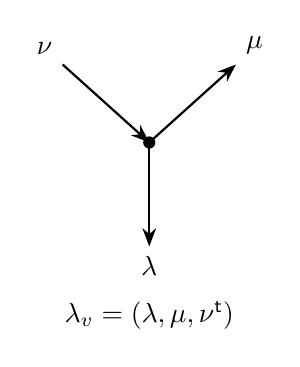
\begin{tikzpicture}[scale=1.1,>=Stealth]
 \coordinate (v) at (0,0);
 \draw[thick,->] (v)--(0,-1.2) node[below] {$\lambda$};
 \draw[thick,->] (v)--(1,0.9) node[above right] {$\mu$};
 \draw[thick,<-] (v)--(-1,0.9) node[above left] {$\nu$};
 \fill (v) circle (2pt);
 \node at (0,-2) {$\lambda_v=(\lambda,\mu,\lt\nu)$};
\end{tikzpicture}
\qquad\qquad
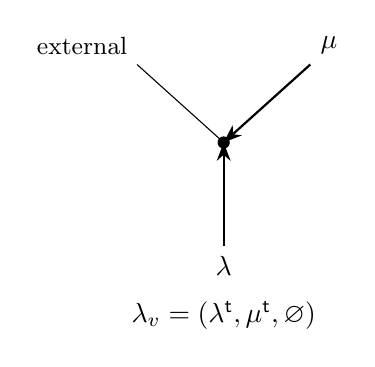
\begin{tikzpicture}[scale=1.1,>=Stealth]
 \coordinate (v) at (0,0);
 \draw[thick,<-] (v)--(0,-1.2) node[below] {$\lambda$};
 \draw[thick,<-] (v)--(1,0.9) node[above right] {$\mu$};
 \draw (v)--(-1,0.9) node[above left] {\small external};
 \fill (v) circle (2pt);
 \node at (0,-2) {$\lambda_v=(\lt\lambda,\lt\mu,\es)$};
\end{tikzpicture}
\end{center}

\begin{lemma}[Directions do not matter]\label{lem:direction}
Reversing the direction of an edge $e$ (which replaces $n_e$ by $-n_e$) and simultaneously
renaming $\lambda_e\rightarrow\lt\lambda_e$ leaves every term of (\ref{eq:Z}) below unchanged.
\end{lemma}
\begin{proof}
The triples at the two endpoints are unchanged by construction. The edge factor becomes
$(-1)^{|\lambda|(-n+1)}q^{-n\kappa(\lt\lambda)/2}=(-1)^{|\lambda|(n+1)}(-1)^{-2n|\lambda|}
q^{n\kappa(\lambda)/2}$, the same as before, by Lemma~\ref{lem:kappa}.
\end{proof}

\subsection{The gluing formula}\label{ssec:gluing}

We are now ready to define the partition function.

\begin{definition}[Partition function {\cite[(4), Def.~2.3]{Kon}}]\label{def:Z}
\begin{equation}\label{eq:Z}
Z=\sum_{(\lambda_e)}\ \prod_{e}(-1)^{|\lambda_e|(n_e+1)}\,q^{n_e\kappa(\lambda_e)/2}\,
Q_e^{|\lambda_e|}\ \prod_{v}C_{\lambda_v}(q),
\end{equation}
the sum running over all assignments of a partition $\lambda_e$ to each internal edge $e$, the
first product over internal edges and the second over nodes. The coefficient
$Z_{\mathbf d}$ of $Q^{\mathbf d}=\prod_eQ_e^{d_e}$ is the (finite) sum over the assignments with
$|\lambda_e|=d_e$ for all $e$. The all-empty assignment contributes $1$.
\end{definition}

\begin{algobox}
\begin{algo}[Partition function from a triangulation]\label{alg:gluing}\ \\
\textbf{Input:} lattice points $\omega_1,\ldots,\omega_N$, a unimodular triangulation, positive
integer weights $w_e$ for the interior segments (all equal to $1$, or the weights of
Section~\ref{ssec:heights}), and a cutoff $D$.\\
\textbf{Output:} all coefficients $Z_{\mathbf d}$ with $\sum_ew_ed_e\le D$.
\begin{enumerate}
\item For every triangle $\sigma$, list its corners counterclockwise and create a node $v_\sigma$.
\item For every interior segment $\tau$ with triangles $\sigma\ni\omega_3$, $\sigma'\ni\omega_3'$:
order its endpoints so that $(\omega_1,\omega_2,\omega_3)$ is ccw, compute
$n=\det(\omega_1,\omega_3',\omega_3)-1$, and direct the edge from $v_\sigma$ to $v_{\sigma'}$ with
label $n_\tau=n$. (Any other choice of direction is allowed, with $n_\tau\rightarrow-n_\tau$.)
\item For every node, record its three sides in ccw order and for each side: boundary, or
(edge $e$, away), or (edge $e$, toward).
\item For every assignment $(\lambda_e)$ with $\sum_e w_e|\lambda_e|\le D$:
 \begin{enumerate}
 \item compute the edge factor $\prod_e(-1)^{|\lambda_e|(n_e+1)}q^{n_e\kappa(\lambda_e)/2}$,
 \item at every node, form the triple $\lambda_v$ of Definition~\ref{def:triple} and compute the
 vertex $C_{\lambda_v}(q)$ from Definition~\ref{def:vertex} (or Table~\ref{tab:vertex}),
 \item add the product of all these to the coefficient of $\prod_eQ_e^{|\lambda_e|}$.
 \end{enumerate}
\item Simplify each coefficient (a rational function of $x=q^{1/2}$).
\end{enumerate}
\end{algo}
\end{algobox}

\begin{remark}
The package implements exactly this algorithm (\texttt{topvertex.partition\_function}), but
organizes step~4 more efficiently: it sums over the partitions of an edge as soon as both of its
endpoints have been processed, which avoids enumerating all assignments at once.
\end{remark}

\begin{remark}[For readers who start from a web]\label{rem:web}
In~\cite{AKMV} the input is a $(p,q)$-web rather than a triangulation: every node carries its
three leg vectors, which are \textit{outgoing} from the node, primitive, sum to zero, and are listed
counterclockwise. The framing can be read off from the web as follows. Let the internal edge $e$
go from the node $a$ to the node $b$. Let $v_k$ be the leg at $a$ that \textit{immediately
precedes} $e$ in counterclockwise order, and $v_{k'}$ the leg at $b$ immediately preceding $e$
in counterclockwise order. Then
\begin{equation}\label{eq:webframing}
n_e=v_{k'}\wedge v_k,\qquad (p_1,q_1)\wedge(p_2,q_2):=p_1q_2-q_1p_2 .
\end{equation}
\textit{Proof:} the leg vectors are the rotated sides (\ref{eq:pq}), and rotation preserves
$\wedge$. In the standard position of Lemma~\ref{lem:framingprops}(3), the side of $\sigma$
preceding $\tau=\omega_1\omega_2$ is $\omega_3\rightarrow\omega_1$, i.e.\ $v_k=\mathrm{rot}(0,-1)$, and the
side of $\sigma'$ preceding $\tau$ (traversed $\omega_2\rightarrow\omega_1$) is $\omega_3'\rightarrow\omega_2$, i.e.\
$v_{k'}=\mathrm{rot}(-n,1)$. Therefore $v_{k'}\wedge v_k=(-n,1)\wedge(0,-1)=n$.
\textit{Example (local $\PP^2$, Figure~\ref{fig:webs}):} the edge from $v_a$ to $v_b$. At $v_a$ the
ccw legs are $(0,-1),(1,1),(-1,0)$ and the edge is $(-1,0)$, so $v_k=(1,1)$. At $v_b$ the ccw legs
are $(1,0),(-2,1),(1,-1)$ and the edge is $(1,0)$, so $v_{k'}=(1,-1)$. Then
$n=(1,-1)\wedge(1,1)=1\cdot1-(-1)\cdot1=2$, in agreement with Example~\ref{ex:framings}. The
comparison with the way this formula is written in~\cite{AKMV} requires care with orientation
conventions, see Appendix~\ref{app:conventions}.
\end{remark}

%=====================================================================================
\section{Worked examples}\label{sec:examples}
%=====================================================================================

In this section we evaluate the formula (\ref{eq:Z}) by hand in three basic examples: a single
edge, local $\PP^2$ and local $\PP^1\times\PP^1$.

\subsection{One edge with framing \texorpdfstring{$n$}{n} and the resolved conifold}\label{ssec:oneedge}

Consider a triangulation with two triangles and one interior segment, with label $n$
(Example~\ref{ex:framings}: the conifold has $n=0$, the $\mathcal O(1)\oplus\mathcal O(-3)$
example has $n=2$). Direct the edge from $v_\sigma$ to $v_{\sigma'}$. The triples are
$(\lambda,\es,\es)$ at the tail and $(\lt\lambda,\es,\es)$ at the head (up to cyclic order), so
by (\ref{eq:C100}) and Theorem~\ref{thm:hook}
\begin{equation}\label{eq:oneedge}
\begin{aligned}
Z_d&=(-1)^{(n+1)d}\sum_{\lambda\vdash d}q^{n\kappa(\lambda)/2}s_\lambda(\qrho)s_{\lt\lambda}(\qrho)\\
&=(-1)^{(n+1)d}\sum_{\lambda\vdash d}q^{(n-1)\kappa(\lambda)/2}s_\lambda(\qrho)^2
=(-1)^{(n+1)d}\sum_{\lambda\vdash d}\frac{q^{n\kappa(\lambda)/2}}{\prod_{s\in\lambda}[h(s)]^2}.
\end{aligned}
\end{equation}

\paragraph{The resolved conifold ($n=0$).} Then $Z_d=(-1)^d\sum_{\lambda\vdash d}\prod_s[h(s)]^{-2}$,
and with the hook lengths of Table~\ref{tab:partitions}:
\begin{align}
Z_1&=-\frac1{[1]^2},\qquad
Z_2=\frac1{[2]^2[1]^2}+\frac1{[2]^2[1]^2}=\frac2{[1]^2[2]^2},\\
Z_3&=-\Big(\frac1{[1]^2[2]^2[3]^2}+\frac1{[1]^4[3]^2}+\frac1{[1]^2[2]^2[3]^2}\Big)
=-\frac{2y+[2]^2}{y\,[1]^2[2]^2[3]^2}=-\frac{y+6}{[1]^2[2]^2[3]^2},
\end{align}
from $\lambda=(3),(2,1),(1,1,1)$ in this order and $[2]^2=y(y+4)$. The package gives (generated):
% GENERATED by notes/make_tables.py from the topvertex package -- do not edit by hand.
% conifold: framing n = 0; checked F_k = -1/(k[k]^2) for k <= 3
\begin{align*}
Z_{1}&=-\frac{1}{[1]^{2}}\\[3pt]
Z_{2}&=\frac{2}{[1]^{2}[2]^{2}}\\[3pt]
Z_{3}&=-\frac{q+q^{-1} + 4}{[1]^{2}[2]^{2}[3]^{2}}=-\frac{y + 6}{[1]^{2}[2]^{2}[3]^{2}}
\end{align*}
\begin{align*}
F_{1}&=-\frac{1}{[1]^{2}}\\[3pt]
F_{2}&=-\frac{1}{2[2]^{2}}\\[3pt]
F_{3}&=-\frac{1}{3[3]^{2}}
\end{align*}
\begin{align*}
y\,f_{1}&=-1&&\Longrightarrow\quad n^{0}_{1}=1\\[3pt]
y\,f_{2}&=0&&\Longrightarrow\quad n^g_{2}=0\ \text{for all }g\\[3pt]
y\,f_{3}&=0&&\Longrightarrow\quad n^g_{3}=0\ \text{for all }g
\end{align*}

The middle block is $F=\log Z$ (Section~\ref{sec:gv}). It suggests the closed formula proved
next. For $F_2$, for example: $F_2=Z_2-\frac12Z_1^2=\frac{2}{y^2(y+4)}-\frac1{2y^2}
=\frac{-y}{2y^2(y+4)}=-\frac1{2[2]^2}$.

\begin{theorem}[Cauchy identities, {\cite[I.4]{Macdonald}}]\label{thm:cauchy}
For two sequences of variables $\vu,\vw$, as formal power series,
\begin{equation}\label{eq:cauchy}
\sum_\lambda s_\lambda(\vu)s_\lambda(\vw)=\prod_{i,j}\frac1{1-u_iw_j},\qquad
\sum_\lambda s_\lambda(\vu)s_{\lt\lambda}(\vw)=\prod_{i,j}(1+u_iw_j).
\end{equation}
\end{theorem}

\begin{proposition}\label{prop:conifold}
For the resolved conifold, $Z=\prod_{k\ge1}(1-Qq^{-k})^{k}$ (expanded in $q^{-1}$) and
\begin{equation}\label{eq:conifoldF}
\log Z=-\sum_{m\ge1}\frac{Q^m}{m[m]^2}.
\end{equation}
For a single edge with $n=1$ (a $(0,-2)$-curve), $Z=\prod_k(1-Qq^{-k})^{-k}$ and
$\log Z=+\sum_m\frac{Q^m}{m[m]^2}$.
\end{proposition}
\begin{proof}
By the first form of (\ref{eq:oneedge}) with $n=0$, $Z=\sum_\lambda s_\lambda(\qrho)
s_{\lt\lambda}(-Q\qrho)$, where $-Q\qrho$ is the sequence $(-Qq^{-i+1/2})_i$ (since $s_\mu$ is
homogeneous of degree $|\mu|$). The second Cauchy identity gives
$Z=\prod_{i,j\ge1}(1-Qq^{-i-j+1})$. Exactly $k$ pairs $(i,j)$ have $i+j-1=k$, so
$Z=\prod_k(1-Qq^{-k})^k$, and
\begin{equation}
\log Z=\sum_kk\log(1-Qq^{-k})=-\sum_k k\sum_m\frac{Q^mq^{-km}}{m}
=-\sum_m\frac{Q^m}{m}\,\frac{q^{-m}}{(1-q^{-m})^2}=-\sum_m\frac{Q^m}{m[m]^2},
\end{equation}
using $\sum_kkt^k=t/(1-t)^2$ and $q^{-m}/(1-q^{-m})^2=1/(q^{m/2}-q^{-m/2})^2$. For $n=1$ the sign is
$(-1)^{2d}=1$ and $Z=\sum_\lambda s_\lambda(\qrho)s_\lambda(Q\qrho)$, so that one can use the first Cauchy
identity. The identities hold as power series in $q^{-1/2}$, but both sides of each
$Q^m$-coefficient are rational functions, so they hold as rational functions.
\end{proof}

\subsection{Local \texorpdfstring{$\PP^2$}{P2}}\label{ssec:P2}

\paragraph{Setup.} The points are $\omega_0=(0,0)$, $\omega_1=(1,0)$, $\omega_2=(0,1)$,
$\omega_3=(-1,-1)$. The triangles are $a=\{\omega_0,\omega_1,\omega_2\}$,
$b=\{\omega_0,\omega_2,\omega_3\}$, $c=\{\omega_0,\omega_3,\omega_1\}$ (ccw). The internal edges
$e_1,e_2,e_3$ cross the segments $\omega_0\omega_1,\omega_0\omega_2,\omega_0\omega_3$. By Example~\ref{ex:framings} each segment
has framings $\pm2$, and we direct the edges so that all labels are $+2$:
\begin{equation}
e_1:\ v_c\rightarrow v_a,\qquad e_2:\ v_a\rightarrow v_b,\qquad e_3:\ v_b\rightarrow v_c,\qquad n_1=n_2=n_3=2
\end{equation}
(Figure~\ref{fig:webs}). The sides of $a$ in ccw order are $\omega_0\omega_1$ ($e_1$, which
points toward $v_a$), $\omega_1\omega_2$ (boundary), $\omega_2\omega_0$ ($e_2$, away from $v_a$).
Doing the same at $b$ and $c$:
\begin{equation}
\lambda_{v_a}=(\lt\lambda_1,\es,\lambda_2),\qquad \lambda_{v_b}=(\lt\lambda_2,\es,\lambda_3),\qquad
\lambda_{v_c}=(\lt\lambda_3,\es,\lambda_1).
\end{equation}
The edge factors are $(-1)^{3|\lambda_i|}q^{2\kappa(\lambda_i)/2}=(-1)^{|\lambda_i|}q^{\kappa(\lambda_i)}$.
All three interior segments represent the same curve class (Section~\ref{sec:classes}), so we
set $Q_1=Q_2=Q_3=Q$:
\begin{equation}\label{eq:ZP2}
Z^{\PP^2}=\sum_{\lambda_1,\lambda_2,\lambda_3}(-Q)^{|\lambda_1|+|\lambda_2|+|\lambda_3|}\,
q^{\kappa(\lambda_1)+\kappa(\lambda_2)+\kappa(\lambda_3)}\,
C_{\lt\lambda_1\es\lambda_2}\,C_{\lt\lambda_2\es\lambda_3}\,C_{\lt\lambda_3\es\lambda_1}.
\end{equation}
We need only vertices with an empty middle slot, $C_{\mu\es\nu}$, given by (\ref{eq:C101}). In
particular, $C_{\mu\es\es}=s_\mu(\qrho)$, $C_{\es\es\nu}=s_\nu(\qrho)$, and
$C_{(1)\es(1)}=(y+1)/y$ (Example~\ref{ex:C110}).

\paragraph{Degree 1.} One of the $\lambda_i$ is $(1)$, the others empty: 3 terms. For
$\lambda_1=(1)$: sign $-1$, $q^0$, $C_{\lambda_{v_a}}=C_{(1)\es\es}=1/[1]$,
$C_{\lambda_{v_b}}=C_{\es\es\es}=1$, $C_{\lambda_{v_c}}=C_{\es\es(1)}=1/[1]$. The other two are the
same by symmetry, so
\begin{equation}
Z_1=-\frac3{[1]^2}=-\frac3y .
\end{equation}

\paragraph{Degree 2.} Either one $\lambda_i$ has size $2$ (3 edges $\times$ 2 partitions $=6$
terms) or two of them are $(1)$ (3 terms):
\begin{center}
\renewcommand{\arraystretch}{1.5}
\begin{tabular}{cccccc}
\toprule
$(\lambda_1,\lambda_2,\lambda_3)$ & sign$\cdot q^{\sum\kappa}$ & $C_{\lambda_{v_a}}$ & $C_{\lambda_{v_b}}$ & $C_{\lambda_{v_c}}$ & term\\
\midrule
$((2),\es,\es)$ & $q^2$ & $C_{(1,1)\es\es}=\frac{q^{-1/2}}{[1][2]}$ & $1$ & $C_{\es\es(2)}=\frac{q^{1/2}}{[1][2]}$ & $\frac{q^2}{[1]^2[2]^2}$\\
$((1,1),\es,\es)$ & $q^{-2}$ & $C_{(2)\es\es}=\frac{q^{1/2}}{[1][2]}$ & $1$ & $C_{\es\es(1,1)}=\frac{q^{-1/2}}{[1][2]}$ & $\frac{q^{-2}}{[1]^2[2]^2}$\\
$((1),(1),\es)$ & $1$ & $C_{(1)\es(1)}=\frac{y+1}{y}$ & $C_{(1)\es\es}=\frac1{[1]}$ & $C_{\es\es(1)}=\frac1{[1]}$ & $\frac{y+1}{y^2}$\\
\midrule
\multicolumn{6}{l}{and the same with $(\lambda_1,\lambda_2,\lambda_3)$ rotated: $(\es,\lambda,\es)$,
$(\es,\es,\lambda)$ and $(\es,(1),(1))$, $((1),\es,(1))$.}\\
\bottomrule
\end{tabular}
\end{center}
(For instance, for $(\es,(1),(1))$ the vertex $C_{(1)\es(1)}$ sits at $v_b$, and for
$((1),\es,(1))$ at $v_c$. The other two vertices are $1/[1]$ each.) Adding up, with
$q^2+q^{-2}=y^2+4y+2$ and $[1]^2[2]^2=y^2(y+4)$:
\begin{equation}\label{eq:Z2P2}
Z_2=\frac{3(q^2+q^{-2})}{[1]^2[2]^2}+\frac{3(q-1+q^{-1})}{[1]^4}
=\frac{3(y^2+4y+2)+3(y+1)(y+4)}{y^2(y+4)}=\frac{6y^2+27y+18}{[1]^2[2]^2}.
\end{equation}

\paragraph{Degree 3.} There are $3\cdot3$ terms with one partition of size $3$, $6\cdot2$ terms
of the form (size $2$, size $1$, empty) in some order, and one term $((1),(1),(1))$: 22 terms.
The package gives (generated, the two lower blocks are explained in Section~\ref{sec:gv}):
% GENERATED by notes/make_tables.py from the topvertex package -- do not edit by hand.
% local P^2: package edges Q0(n=-2,class=(-3, 1, 1, 1)), Q1(n=2,class=(-3, 1, 1, 1)), Q2(n=2,class=(-3, 1, 1, 1))
\begin{align*}
Z_{1}&=-\frac{3}{[1]^{2}}\\[3pt]
Z_{2}&=\frac{6(q^{2}+q^{-2}) + 3(q+q^{-1})}{[1]^{2}[2]^{2}}=\frac{6y^{2} + 27y + 18}{[1]^{2}[2]^{2}}\\[3pt]
Z_{3}&=-\frac{10(q^{6}+q^{-6}) + 7(q^{5}+q^{-5}) + 8(q^{4}+q^{-4}) + 3(q^{3}+q^{-3}) + 10(q^{2}+q^{-2}) + 26(q+q^{-1}) + 34}{[1]^{2}[2]^{2}[3]^{2}}\\&=-\frac{10y^{6} + 127y^{5} + 618y^{4} + 1432y^{3} + 1588y^{2} + 756y + 162}{[1]^{2}[2]^{2}[3]^{2}}
\end{align*}
\begin{align*}
F_{1}&=-\frac{3}{[1]^{2}}\\[3pt]
F_{2}&=\frac{12(q+q^{-1}) + 21}{2[2]^{2}}=\frac{12y + 45}{2[2]^{2}}\\[3pt]
F_{3}&=-\frac{10(q^{3}+q^{-3}) + 27(q^{2}+q^{-2}) + 54(q+q^{-1}) + 62}{[3]^{2}}\\&=-\frac{10y^{3} + 87y^{2} + 252y + 244}{[3]^{2}}
\end{align*}
\begin{align*}
y\,f_{1}&=-3&&\Longrightarrow\quad n^{0}_{1}=3\\[3pt]
y\,f_{2}&=6&&\Longrightarrow\quad n^{0}_{2}=-6\\[3pt]
y\,f_{3}&=-10y - 27&&\Longrightarrow\quad n^{0}_{3}=27,\ n^{1}_{3}=-10
\end{align*}

The first two lines agree with our hand computation.

\subsection{Local \texorpdfstring{$\PP^1\times\PP^1$}{P1xP1}}\label{ssec:F0}

\paragraph{Setup.} The points are $\omega_0=(0,0)$ and
$\omega_1,\ldots,\omega_4=(1,0),(0,1),(-1,0),(0,-1)$. The triangles are
$k=\{\omega_0,\omega_k,\omega_{k+1}\}$ (indices mod 4). The internal edge $e_k$ crosses
$\omega_0\omega_k$ and lies between the triangles $k-1$ and $k$. By Example~\ref{ex:framings} the framing of
$e_k$ is $-1$ at triangle $k$ and $+1$ at triangle $k-1$, so we direct $e_k$ from $v_{k-1}$ to
$v_k$ with label $n_k=1$ (Figure~\ref{fig:webs}). At $v_k$ the ccw sides are
$\omega_0\omega_k$ ($e_k$, toward $v_k$), $\omega_k\omega_{k+1}$ (boundary) and
$\omega_{k+1}\omega_0$ ($e_{k+1}$, away), so $\lambda_{v_k}=(\lt\lambda_k,\es,\lambda_{k+1})$. The edge
factors are $(-1)^{2|\lambda_k|}q^{\kappa(\lambda_k)/2}=q^{\kappa(\lambda_k)/2}$. The segments
$\omega_0\omega_1$ and $\omega_0\omega_3$ represent one curve class $B$, and $\omega_0\omega_2$,
$\omega_0\omega_4$ another class $F$ (Section~\ref{sec:classes}). Therefore we set
$Q_1=Q_3=Q_B$, $Q_2=Q_4=Q_F$:
\begin{equation}
Z^{\PP^1\times\PP^1}=\sum_{\lambda_1,\ldots,\lambda_4}Q_B^{|\lambda_1|+|\lambda_3|}Q_F^{|\lambda_2|+|\lambda_4|}
\prod_{k=1}^4q^{\kappa(\lambda_k)/2}\,C_{\lt\lambda_k\es\lambda_{k+1}}\qquad(\lambda_5=\lambda_1).
\end{equation}

\paragraph{Total degree $\le2$.} We write $Z_{(d_B,d_F)}$ for the coefficient of $Q_B^{d_B}Q_F^{d_F}$.
\begin{itemize}
\item $(1,0)$: $\lambda_1=(1)$ or $\lambda_3=(1)$. For $\lambda_1=(1)$: $C_{\lambda_{v_1}}=C_{(1)\es\es}$,
$C_{\lambda_{v_4}}=C_{\es\es(1)}$, giving $1/y$. Therefore $Z_{(1,0)}=2/y$, and likewise $Z_{(0,1)}=2/y$.
\item $(2,0)$: (i) $\lambda_1=\mu\vdash2$, others empty: $q^{\kappa(\mu)/2}C_{\lt\mu\es\es}C_{\es\es\mu}
=q^{\kappa(\mu)/2}s_{\lt\mu}(\qrho)s_\mu(\qrho)=s_\mu(\qrho)^2$, which gives
$\frac{q+q^{-1}}{[1]^2[2]^2}$ summed over $\mu=(2),(1,1)$, (ii) the same for $\lambda_3$, (iii)
$\lambda_1=\lambda_3=(1)$: the four vertices are $C_{(1)\es\es},C_{\es\es(1)},C_{(1)\es\es},C_{\es\es(1)}$,
giving $1/y^2$. Altogether
\begin{equation}
Z_{(2,0)}=\frac{2(q+q^{-1})}{[1]^2[2]^2}+\frac1{[1]^4}=\frac{2(y+2)+(y+4)}{y^2(y+4)}=\frac{3y+8}{[1]^2[2]^2},
\end{equation}
and the same for $Z_{(0,2)}$.
\item $(1,1)$: one $B$-edge and one $F$-edge carry $(1)$. All four such pairs are adjacent
(they share a node), e.g.\ $\lambda_1=\lambda_2=(1)$ gives $C_{\lambda_{v_1}}=C_{(1)\es(1)}=\frac{y+1}y$,
$C_{\lambda_{v_2}}=C_{(1)\es\es}$, $C_{\lambda_{v_4}}=C_{\es\es(1)}$, $C_{\lambda_{v_3}}=1$. Therefore
$Z_{(1,1)}=4\,\frac{y+1}{y^2}$.
\end{itemize}
The package gives (generated):
% GENERATED by notes/make_tables.py from the topvertex package -- do not edit by hand.
% local F0: package edges Q0(n=-1,class=(-2, 0, 1, 0, 1)), Q1(n=1,class=(-2, 1, 0, 1, 0)), Q2(n=1,class=(-2, 0, 1, 0, 1)), Q3(n=1,class=(-2, 1, 0, 1, 0)); B = spokes to (+-1,0), F = spokes to (0,+-1)
\begin{align*}
Z_{(1,0)}&=\frac{2}{[1]^{2}}\\[3pt]
Z_{(0,1)}&=\frac{2}{[1]^{2}}\\[3pt]
Z_{(2,0)}&=\frac{3(q+q^{-1}) + 2}{[1]^{2}[2]^{2}}=\frac{3y + 8}{[1]^{2}[2]^{2}}\\[3pt]
Z_{(1,1)}&=\frac{4(q+q^{-1}) - 4}{[1]^{4}}=\frac{4y + 4}{[1]^{4}}\\[3pt]
Z_{(0,2)}&=\frac{3(q+q^{-1}) + 2}{[1]^{2}[2]^{2}}=\frac{3y + 8}{[1]^{2}[2]^{2}}
\end{align*}
\begin{align*}
F_{(1,0)}&=\frac{2}{[1]^{2}}\\[3pt]
F_{(0,1)}&=\frac{2}{[1]^{2}}\\[3pt]
F_{(2,0)}&=\frac{1}{[2]^{2}}\\[3pt]
F_{(1,1)}&=\frac{4}{[1]^{2}}\\[3pt]
F_{(0,2)}&=\frac{1}{[2]^{2}}
\end{align*}
\begin{align*}
y\,f_{(1,0)}&=2&&\Longrightarrow\quad n^{0}_{(1,0)}=-2\\[3pt]
y\,f_{(0,1)}&=2&&\Longrightarrow\quad n^{0}_{(0,1)}=-2\\[3pt]
y\,f_{(2,0)}&=0&&\Longrightarrow\quad n^g_{(2,0)}=0\ \text{for all }g\\[3pt]
y\,f_{(1,1)}&=4&&\Longrightarrow\quad n^{0}_{(1,1)}=-4\\[3pt]
y\,f_{(0,2)}&=0&&\Longrightarrow\quad n^g_{(0,2)}=0\ \text{for all }g
\end{align*}


\begin{remark}[Local toric surfaces in general]\label{rem:chain}
The two examples above are instances of a general pattern~\cite[\S2.5.2]{Kon}. If the polygon
has a single interior point $\omega_0$ and the boundary points $\omega_1,\ldots,\omega_r$ are
listed counterclockwise, the triangulation is the ``star'' $\{\omega_0,\omega_k,\omega_{k+1}\}$
and the same reasoning gives
\begin{equation}\label{eq:chain}
Z=\sum_{\lambda_1,\ldots,\lambda_r}\prod_{k=1}^r(-1)^{(m_k+1)|\lambda_k|}q^{m_k\kappa(\lambda_k)/2}
Q_k^{|\lambda_k|}\,C_{\lt\lambda_k\es\lambda_{k+1}},\qquad m_k=1-\det(\omega_0,\omega_{k-1},\omega_{k+1}),
\end{equation}
where $e_k$ is directed from triangle $k-1$ to triangle $k$ and $m_k$ is its label. Local $\PP^2$
has $m=(2,2,2)$, local $\PP^1\times\PP^1$ has $m=(1,1,1,1)$, and local $F_1$ (with the points of
Example~\ref{ex:framings}) has $m=(0,1,2,1)$.
\end{remark}

\begin{physrem}
For a star triangulation, $X$ is the total space of the canonical bundle of a compact toric
surface $S$, and $e_k$ is a curve $C_k\subset S$ with self-intersection $C_k\cdot C_k=m_k-1$:
lines in $\PP^2$ have self-intersection $+1$, the rulings of $\PP^1\times\PP^1$ have $0$, and
$F_1$ has curves with $-1$ (the exceptional curve), $0$ (fibers) and $+1$.
\end{physrem}

\begin{exercise}\label{ex:ex1}
Using only $Z_1,Z_2,Z_3$ of the conifold computed by hand above and $\log(1+W)=W-W^2/2+W^3/3-\ldots$,
check that $F_3=Z_3-Z_1Z_2+\frac13Z_1^3=-\frac1{3[3]^2}$. (Use $[3]^2=y(y+3)^2$.)
\end{exercise}

\begin{exercise}\label{ex:ex2}
For local $F_1$, use (\ref{eq:chain}) with $m=(0,1,2,1)$ and $Q_1=Q_B$, $Q_2=Q_4=Q_F$,
$Q_3=Q_BQ_F$ (Section~\ref{sec:classes}) to compute the coefficients $Z_B$ of $Q_B$ and $Z_{B+F}$ of
$Q_BQ_F$, and $F_{B+F}=Z_{B+F}-Z_BZ_F$. (After Section~\ref{sec:gv} one will be able to read
off $n^0_B=1$ and $n^0_{B+F}=3$.)
\end{exercise}

\begin{exercise}\label{ex:ex3}
For local $\PP^2$, compute the contribution to $Z_3$ of the 9 terms in which a single
$\lambda_i$ has size 3.
\end{exercise}

%=====================================================================================
\section{Free energy and Gopakumar-Vafa invariants}\label{sec:gv}
%=====================================================================================

In this section we define the free energy and the Gopakumar-Vafa invariants, and describe how
the invariants are extracted from $Z$.


\subsection{The free energy}

After identifying the variables according to curve classes (Section~\ref{sec:classes}), $Z$ is
a power series $Z=1+\sum_{\beta\ne0}Z_\beta Q^\beta$ in variables $Q=(Q_1,\ldots,Q_r)$, where
$\beta=(\beta_1,\ldots,\beta_r)$ runs over vectors of non-negative integers (``degrees'' or
``classes'') and $Q^\beta=\prod_iQ_i^{\beta_i}$. Write $Z=1+W$.

\begin{definition}
The \textit{free energy} is $F=\log Z=\sum_{m\ge1}\frac{(-1)^{m+1}}{m}W^m=\sum_{\beta\ne0}F_\beta Q^\beta$.
\end{definition}

Since $W$ has no constant term, only finitely many $m$ contribute to each $F_\beta$ (at most the
total degree of $\beta$). For one variable:
\begin{equation}
F_1=Z_1,\qquad F_2=Z_2-\tfrac12Z_1^2,\qquad F_3=Z_3-Z_1Z_2+\tfrac13Z_1^3 .
\end{equation}
For two variables one has, for example, $F_{(1,1)}=Z_{(1,1)}-Z_{(1,0)}Z_{(0,1)}$ and
$F_{(2,0)}=Z_{(2,0)}-\frac12Z_{(1,0)}^2$.

\subsection{The Gopakumar-Vafa expansion}

\begin{definition}[GV invariants, physical convention]
The \textit{Gopakumar-Vafa invariants} $n^g_\beta$ ($g\ge0$, $\beta\ne0$) are the numbers defined by
\begin{equation}\label{eq:GV}
F=\sum_{\beta\ne0}\ \sum_{g\ge0}\ \sum_{k\ge1}\ n^g_\beta\,(-1)^{g-1}\,\frac1k\,[k]^{2g-2}\,Q^{k\beta}.
\end{equation}
\end{definition}

The existence of such numbers, their integrality, and the fact that for each $\beta$ only
finitely many $g$ have $n^g_\beta\neq0$ is a theorem. It was proved in exactly the combinatorial
setting of these notes, by Peng~\cite{Peng} for local surfaces and by Konishi~\cite{Kon} in
general. The algorithm below
computes the $n^g_\beta$ and, along the way, checks these properties.

\begin{physrem}
In physics $q=e^{ig_s}$ with $g_s$ the string coupling, and $F=\sum_g g_s^{2g-2}F_g(Q)$ is the
genus expansion of the topological string free energy. Gopakumar and Vafa~\cite{GV} argued that
$F$ has the form $\sum n^g_\beta\frac1k\big(2\sin\frac{kg_s}2\big)^{2g-2}Q^{k\beta}$. Here
$n^g_\beta$ counts (with signs) BPS states of M2-branes wrapping curves of class $\beta$ and
``genus'' $g$, and the sum over $k$ accounts for $k$-fold multiple covers. With $q=e^{ig_s}$ we
have $[k]=q^{k/2}-q^{-k/2}=2i\sin\frac{kg_s}2$, so $\big(2\sin\frac{kg_s}2\big)^2=-[k]^2$ and
$\big(2\sin\frac{kg_s}2\big)^{2g-2}=(-1)^{g-1}[k]^{2g-2}$, which is (\ref{eq:GV}). The leading power
$[k]^{-2}\sim(kg_s)^{-2}$ for $g=0$ is the genus-zero contribution, and higher $g$ come with more
powers of $g_s$. The variable $y=[1]^2=-4\sin^2\frac{g_s}2$ is the natural expansion parameter.
\end{physrem}

\subsection{Extracting the integers}

Fix $\beta$ and suppose all $n^g_{\beta'}$ for classes $\beta'=\beta/k$ ($k\ge2$, $k\mid\beta$, meaning
$k$ divides every component of $\beta$) are already known. In (\ref{eq:GV}) the coefficient of
$Q^\beta$ receives contributions from $(\beta,k=1)$ and from $(\beta/k,k)$. Define
\begin{equation}\label{eq:fbeta}
f_\beta=F_\beta-\sum_{k\ge2,\ k\mid\beta}\ \frac1k\sum_gn^g_{\beta/k}(-1)^{g-1}[k]^{2g-2}.
\end{equation}
Then $f_\beta=\sum_gn^g_\beta(-1)^{g-1}[1]^{2g-2}$, i.e.
\begin{equation}\label{eq:Pbeta}
P_\beta:=y\,f_\beta=\sum_{g\ge0}n^g_\beta(-1)^{g-1}y^g,\qquad y=[1]^2=q-2+q^{-1}.
\end{equation}

\begin{algobox}
\begin{algo}[GV extraction]\label{alg:gv}\ \\
\textbf{Input:} $F_\beta$ for all $\beta$ up to some degree. \textbf{Output:} $n^g_\beta$.\\
Process the classes $\beta$ in order of increasing degree. For each $\beta$:
\begin{enumerate}
\item Compute $f_\beta$ by (\ref{eq:fbeta}) (the subtracted terms use invariants of smaller classes).
\item Compute $P_\beta=y\,f_\beta$ and simplify. \textit{Check:} $P_\beta$ is a Laurent polynomial
in $q$ (no denominators, integral powers of $q$) and $P_\beta(q)=P_\beta(1/q)$.
\item Write $P_\beta$ as a polynomial in $y$ by peeling off the top power: if the highest power
of $q$ in $P_\beta$ is $q^G$ with coefficient $c_G$, subtract $c_Gy^G$ (the top term of $y^G$ is $q^G$)
and repeat (Exercise~\ref{ex:ypoly}).
\item If $P_\beta=\sum_gc_gy^g$, then $n^g_\beta=(-1)^{g-1}c_g$. \textit{Check:} integers.
\end{enumerate}
\end{algo}
\end{algobox}

\subsection{Examples}

\paragraph{Conifold.} By Proposition~\ref{prop:conifold}, $F_m=-\frac1{m[m]^2}$. For $\beta=1$:
$P_1=yF_1=-1=n^0_1(-1)^{-1}$, so $n^0_1=1$. For $\beta=m\ge2$: $f_m=F_m-\frac1m n^0_1(-1)^{-1}[m]^{-2}=0$,
so $n^g_m=0$. The conifold has a single BPS state: one rigid sphere.

\paragraph{Local $\PP^2$, degree 1.} $F_1=Z_1=-3/y$, so $P_1=-3$ and $n^0_1=3$: the three
``lines'' $e_1,e_2,e_3$ each contribute one. (Geometrically, the lines in $\PP^2$ form a
2-dimensional family, and $n^0_1=3$ is its signed Euler characteristic.)

\paragraph{Local $\PP^2$, degree 2.} From $Z_1=-3/y$ and (\ref{eq:Z2P2}),
\begin{equation}
F_2=Z_2-\tfrac12Z_1^2=\frac{6y^2+27y+18}{y^2(y+4)}-\frac{9}{2y^2}
=\frac{12y^2+54y+36-9y-36}{2y^2(y+4)}=\frac{12y+45}{2y(y+4)} .
\end{equation}
The class $2=2\cdot1$ is divisible by $k=2$, and $n^0_1=3$, so the multicover subtraction is
\begin{equation}
f_2=F_2-\frac12\,n^0_1\,(-1)^{-1}[2]^{-2}=F_2+\frac{3}{2y(y+4)}=\frac{12y+48}{2y(y+4)}=\frac6y .
\end{equation}
Therefore $P_2=y f_2=6=n^0_2(-1)^{-1}$, i.e.\ $n^0_2=-6$, and $n^g_2=0$ for $g\ge1$. Note how the
denominator $y+4$ (coming from $[2]^2$) cancels only after the subtraction: this is the
integrality theorem at work.

\paragraph{Local $\PP^2$, degree 3.} Here $k=3$ divides $3$, and $f_3=F_3-\frac13n^0_1(-1)^{-1}[3]^{-2}
=F_3+\frac1{[3]^2}$. With $F_3$ from the generated block in Section~\ref{ssec:P2} one finds
$P_3=yf_3=-10y-27$, so $n^0_3=(-1)^{1}\cdot(-27)=27$ and $n^1_3=(-1)^0\cdot(-10)=-10$. This is the
first genus-one invariant: plane cubics are elliptic curves.

\paragraph{Local $\PP^1\times\PP^1$.} From Section~\ref{ssec:F0}: $F_{(1,0)}=2/y$, so $n^0_{(1,0)}=-2$
(a $\PP^1$-family of $(0,-2)$-curves: signed Euler characteristic $-2$). Next
$F_{(2,0)}=Z_{(2,0)}-\frac12Z_{(1,0)}^2=\frac{3y+8}{y^2(y+4)}-\frac2{y^2}=\frac{1}{y(y+4)}=\frac1{[2]^2}$,
and $f_{(2,0)}=F_{(2,0)}-\frac12(-2)(-1)[2]^{-2}=0$, so $n^g_{(2,0)}=0$. Finally
$F_{(1,1)}=Z_{(1,1)}-Z_{(1,0)}Z_{(0,1)}=\frac{4(y+1)}{y^2}-\frac4{y^2}=\frac4y$ (no multicover term,
since $(1,1)$ is not divisible by any $k\ge2$), so $n^0_{(1,1)}=-4$.

\subsection{Tables}

Table~\ref{tab:gv} lists the invariants of local $\PP^2$ up to degree 5 and the genus-zero
invariants of local $\PP^1\times\PP^1$ up to bidegree $(3,3)$, as given in the literature
(KKV~\cite{KKV}, Table~4, and CKYZ~\cite{CKYZ}, Table~9, in the physical convention). The package
reproduces all of them from Algorithm~\ref{alg:gluing} and Algorithm~\ref{alg:gv} (its test suite
compares with these numbers, stored in \texttt{tests/data.py}).

\begin{table}[ht]
\centering
% GENERATED by notes/make_tables.py from the topvertex package -- do not edit by hand.
\begin{tabular}{c|rrrrrrr}
\toprule
$d$ & $g=0$ & $g=1$ & $g=2$ & $g=3$ & $g=4$ & $g=5$ & $g=6$\\
\midrule
$1$ & $3$ & $0$ & $0$ & $0$ & $0$ & $0$ & $0$\\
$2$ & $-6$ & $0$ & $0$ & $0$ & $0$ & $0$ & $0$\\
$3$ & $27$ & $-10$ & $0$ & $0$ & $0$ & $0$ & $0$\\
$4$ & $-192$ & $231$ & $-102$ & $15$ & $0$ & $0$ & $0$\\
$5$ & $1695$ & $-4452$ & $5430$ & $-3672$ & $1386$ & $-270$ & $21$\\
\bottomrule
\end{tabular}
\qquad
\begin{tabular}{c|rrrr}
\toprule
$d_B\backslash d_F$ & $0$ & $1$ & $2$ & $3$\\
\midrule
$0$ & -- & $-2$ & $0$ & $0$\\
$1$ & $-2$ & $-4$ & $-6$ & $-8$\\
$2$ & $0$ & $-6$ & $-32$ & $-110$\\
$3$ & $0$ & $-8$ & $-110$ & $-756$\\
\bottomrule
\end{tabular}

\caption{(Generated from \texttt{tests/data.py}.) Left: $n^g_d$ for local $\PP^2$, $d\le5$,
all genera (all $n^g_d$ not shown vanish, and the top genus $g=(d-1)(d-2)/2$ has
$n^g_d=(-1)^{d(d+3)/2}\big(\tfrac{d(d+3)}2+1\big)$, e.g.\ $n^6_5=21$). Right: $n^0_{(d_B,d_F)}$ for local
$\PP^1\times\PP^1$, symmetric under $d_B\leftrightarrow d_F$.}
\label{tab:gv}
\end{table}

%=====================================================================================
\section{Curve classes and truncation}\label{sec:classes}
%=====================================================================================

In this section we explain which of the variables $Q_e$ have to be identified, and how the sum
(\ref{eq:Z}) is truncated.


\subsection{The class of an edge}

Let $\omega_1,\ldots,\omega_N$ be all the lattice points of the polygon (in some fixed order) and
$\hatw_i=(a_i,b_i,1)$.

\begin{definition}
The \textit{relation lattice} is $L=\{l\in\Z^N:\ \sum_il_i\hatw_i=0\}$. For an interior segment
$\tau$, with $\omega_1,\omega_2,\omega_3,\omega_3'$ and $a_1,a_2$ as in Lemma~\ref{lem:a1a2}, the
\textit{relation vector} (or \textit{class}) $l_\tau\in L$ has entries $a_1$ at $\omega_1$, $a_2$ at
$\omega_2$, $+1$ at $\omega_3$ and at $\omega_3'$, and $0$ elsewhere. The statement $l_\tau\in L$ is
precisely the relation (\ref{eq:relation}).
\end{definition}

The vector $l_\tau$ does not depend on which of the two flags is used (the two choices exchange
$\omega_1\leftrightarrow\omega_2$, $a_1\leftrightarrow a_2$ and $\omega_3\leftrightarrow\omega_3'$).
Since the $\hatw_i$ span a space of dimension 3, $L$ has rank $N-3$.

\begin{physrem}
$L\cong H_2(X;\Z)$, and $l_\tau$ is the homology class of the curve $C_\tau$: its entries are the
intersection numbers of $C_\tau$ with the toric divisors $D_i$ (one per lattice point). For the
interior point $\omega_0$ of a star triangulation, $D_0$ is the compact surface $S$ and
the entry of $l_\tau$ at $\omega_0$ is $-(\text{self-intersection of $C_\tau$ in $S$})-2$, consistent with
Remark~\ref{rem:chain} (e.g.\ $-3$ for a line in $\PP^2$).
\end{physrem}

The term of (\ref{eq:Z}) with partitions $(\lambda_\tau)$ describes curves in the class
$\beta=\sum_\tau|\lambda_\tau|\,l_\tau\in L$. Therefore, after choosing a basis $b_1,\ldots,b_r$ of $L$
($r=N-3$) and writing $l_\tau=\sum_ic_{\tau i}b_i$, we substitute
\begin{equation}\label{eq:subst}
Q_\tau\ \longmapsto\ \prod_{i=1}^rQ_i^{c_{\tau i}} .
\end{equation}
Since (\ref{eq:subst}) is a ring homomorphism it commutes with $\log$, so it may be done before
or after taking $F=\log Z$ (in \cite[(8)]{Kon} the logarithm is taken first, and then one sums
over the degree vectors in a given class).

\begin{example}\label{ex:classes}
\begin{itemize}
\item \textit{Local $\PP^2$} (points $\omega_0,\ldots,\omega_3$ as in Section~\ref{ssec:P2}). For
$\tau=\omega_0\omega_1$ we found $\omega_3'=-a_1\omega_0-a_2\omega_1-\omega_2$ with $a_1=-3$
(at $\omega_0$) and $a_2=1$ (at $\omega_1$), so $l=(-3,1,1,1)$. One can check that
$-3(0,0,1)+(1,0,1)+(0,1,1)+(-1,-1,1)=0$. By symmetry all three segments have the same class $H$
(the line in $\PP^2$), so $Q_1=Q_2=Q_3=Q$.
\item \textit{Local $\PP^1\times\PP^1$.} Here $l(\omega_0\omega_1)=l(\omega_0\omega_3)=(-2,0,1,0,1)$ and
$l(\omega_0\omega_2)=l(\omega_0\omega_4)=(-2,1,0,1,0)$. The rank is $5-3=2$, with two classes $B$
and $F$, and
$Q_1=Q_3=Q_B$, $Q_2=Q_4=Q_F$.
\item \textit{Local $F_1$} (points $\omega_0,\ldots,\omega_4=(0,0),(0,1),(-1,1),(0,-1),(1,0)$):
\begin{equation}
l_1=(-1,-1,1,0,1),\quad l_2=l_4=(-2,1,0,1,0),\quad l_3=(-3,0,1,1,1)=l_1+l_2 .
\end{equation}
Therefore, with $B=l_1$ (the $(-1)$-curve) and $F=l_2$ (the fiber), the four edges have classes
$B,F,B+F,F$, and $Q_1=Q_B$, $Q_2=Q_4=Q_F$, $Q_3=Q_BQ_F$.
\end{itemize}
\end{example}

\subsection{Truncation needs positive weights}

To compute $F_\beta$ we need \textit{all} assignments $(\lambda_\tau)$ with
$\sum_\tau|\lambda_\tau|l_\tau=\beta$, and we need the products in $\log Z$ to be complete. The
naive cutoff ``total edge degree $\sum_\tau|\lambda_\tau|\le D$'' is not adapted to classes:

\begin{example}[Local $F_1$]\label{ex:F1trunc}
The class $B+F$ arises from $\lambda_3=(1)$ (edge degree $1$) and from
$\lambda_1=\lambda_2=(1)$ or $\lambda_1=\lambda_4=(1)$ (edge degree $2$). With the cutoff
``edge degree $\le1$'' one would get $F_{B+F}=Z_{B+F}=-1/y$ and conclude $n^0_{B+F}=1$. The
correct value, using all terms (Exercise~\ref{ex:ex2}), is $F_{B+F}=-3/y$ and $n^0_{B+F}=3$.
\end{example}

The cure is to give each edge a positive \textit{weight} $w_\tau$ that is a linear function of its
class, and truncate by $\sum_\tau w_\tau|\lambda_\tau|\le D$. Then the weight
$w(\beta)$ of a class is well defined, the truncation keeps exactly the classes with
$w(\beta)\le D$, and keeps them completely. Moreover, since all $w_\tau>0$, each class receives
only finitely many terms.

Such weights are provided by heights of the triangulation (Definition~\ref{def:heights}).
Namely, for heights $h_1,\ldots,h_N$ take
\begin{equation}\label{eq:weights}
w_\tau:=\langle h,l_\tau\rangle=\sum_ih_i\,(l_\tau)_i .
\end{equation}
This is the weight of $\tau$ introduced in Section~\ref{ssec:heights}. To see this, let $\phi$
be the affine function on $\sigma$ with $\phi(\omega_i)=h_i$ at its corners. Then
$\sum_i(l_\tau)_i\phi(\omega_i)=0$ because $l_\tau\in L$, so that
$\langle h,l_\tau\rangle=h(\omega_3')-\phi(\omega_3')$. This is the height of the lifted fourth
point above the plane through the lifted triangle $\sigma$. In particular, the integers
$h_1,\ldots,h_N$ are heights of the triangulation if and only if $w_\tau>0$ for all interior
segments $\tau$. The weights are linear in the class by construction. With the heights $h=0$ at
the interior point and $h=1$ at the boundary points (Example~\ref{ex:heights}), which can also
be used for local $F_1$, one gets
\begin{equation}
\PP^2:\ w=3,\qquad \PP^1\times\PP^1:\ w_B=w_F=2,\qquad F_1:\ w_B=1,\ w_F=2,\ w_{B+F}=3 .
\end{equation}
For $F_1$ the truncation $\sum w_\tau|\lambda_\tau|\le3$ contains the class $B+F$ completely.
The package uses the weights (\ref{eq:weights}) by default, with the heights found as described
in Section~\ref{ssec:heights}.

\begin{physrem}
$w_\tau$ is the area of the curve $C_\tau$ for the K\"ahler class determined by $h$, and
regularity of the triangulation is the statement that $X$ admits a K\"ahler metric (it is a
projective morphism over the singular affine toric variety). Truncating by area is natural:
$Q^\beta=e^{-t(\beta)}$.
\end{physrem}

%=====================================================================================
\appendix
\section{Cross-check: the 5d Nekrasov partition function}\label{app:nekrasov}
%=====================================================================================

In this appendix we compare the vertex partition function with a completely different formula:
the Nekrasov instanton partition function of a 5d gauge theory~\cite{Nekrasov,IKP-SUN}. The
comparison is possible for a large class of triangulations. The gauge theories that appear are \textit{linear quivers}:
the gauge group is $U(N_1)\times\ldots\times U(N_r)$, with bifundamental matter between
consecutive factors, fundamental matter at the two ends, and Chern-Simons terms. The dictionary
between the triangulation and the gauge theory given below was read off from the dual graph and
verified by computer (\texttt{topvertex.nekrasov}). It is not taken from the literature.

\paragraph{Ladder triangulations.} Call a triangulation a \textit{ladder} along a primitive
vector $d$ if every triangle has a side parallel to $d$. After an orientation-preserving
unimodular change of coordinates we may take $d=(0,1)$. The lattice points of the polygon are
then arranged in columns $X=0,1,\ldots,r+1$,
\begin{equation}
\text{column } i:\qquad \omega^{(i)}_j=(i,\,b_i+j),\qquad j=0,\ldots,N_i .
\end{equation}
The triangulation contains all the vertical unit segments $\omega^{(i)}_{k-1}\omega^{(i)}_k$,
and every strip between two adjacent columns is cut into triangles that have one vertical side
and the opposite corner in the other column (Figure~\ref{fig:quiver}). We assume $r\ge1$.

\begin{figure}[ht]
\centering
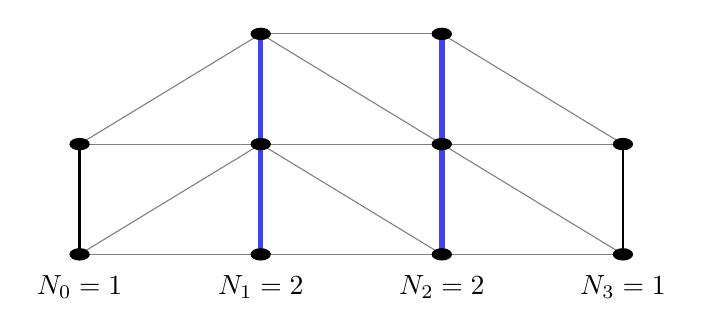
\begin{tikzpicture}[xscale=2.3,yscale=1.4]
  \foreach \a/\b/\c/\d in {0/0/1/0, 1/0/2/0, 2/0/3/0, 0/1/1/2, 1/2/2/2, 2/2/3/1,
                           0/0/1/1, 0/1/1/1, 1/1/2/0, 1/1/2/1, 1/2/2/1, 2/1/3/0, 2/1/3/1}
    \draw[gray] (\a,\b) -- (\c,\d);
  \foreach \a/\b/\c/\d in {0/0/0/1, 3/0/3/1} \draw[thick] (\a,\b) -- (\c,\d);
  \foreach \a/\b/\c/\d in {1/0/1/1, 1/1/1/2, 2/0/2/1, 2/1/2/2} \draw[line width=2pt, blue!75] (\a,\b) -- (\c,\d);
  \foreach \p in {(0,0),(0,1),(1,0),(1,1),(1,2),(2,0),(2,1),(2,2),(3,0),(3,1)} \fill \p circle (1.6pt);
  \node[below] at (0,-0.1) {$N_0=1$};
  \node[below] at (1,-0.1) {$N_1=2$};
  \node[below] at (2,-0.1) {$N_2=2$};
  \node[below] at (3,-0.1) {$N_3=1$};
\end{tikzpicture}
\caption{A ladder triangulation with $r=2$ and all $b_i=0$: the gauge theory is
$U(2)\times U(2)$ with one bifundamental and one fundamental hypermultiplet at each end, and
$\kappa_1=\kappa_2=-\tfrac12$. The four thick blue segments are the gauge branes. They are dual
to the horizontal edges that carry the partitions $Y^{(i)}_k$.}\label{fig:quiver}
\end{figure}

\paragraph{The gauge theory.} The columns $1,\ldots,r$ are the gauge groups $U(N_i)$. Two
adjacent gauge columns are joined by a bifundamental hypermultiplet. The columns $0$ and $r+1$ give $N_0$
and $N_{r+1}$ fundamental hypermultiplets of the first and of the last group (none if the column
is a single point). In the dual graph the vertical segment $\omega^{(i)}_{k-1}\omega^{(i)}_k$ is
a horizontal edge, which we call the \textit{brane} $(i,k)$, $k=1,\ldots,N_i$ counted from the
bottom. For $1\le i\le r$ it is an internal edge, of class $T_{i,k}$, and it carries a partition
$Y^{(i)}_k$. For $i=0,r+1$ it is an external leg and we put $Y^{(i)}_k=\es$.

The position of the brane $(i,k)$ is the vector
\begin{equation}
y^{(i)}_k=e_{\omega^{(i)}_k}-e_{\omega^{(i)}_{k-1}}\in\Z^{\#\text{points}},\qquad\text{so that}\qquad
\langle h,y^{(i)}_k\rangle=h(\omega^{(i)}_k)-h(\omega^{(i)}_{k-1})
\end{equation}
for heights $h$ of the triangulation (Section~\ref{ssec:heights}). Two facts make this useful.
First, the difference $y-y'$ of two branes in the same column or in adjacent columns is a
relation vector, and therefore a curve class. We write $Q^{y-y'}$ for the corresponding
monomial.
Second, its K\"ahler weight $\langle h,y-y'\rangle$ is never zero, and its sign does not depend on
the choice of $h$. Namely, the triangles of a strip are ordered from bottom to top, and each of
them contains exactly one brane. Two consecutive triangles are separated by a diagonal segment
$\tau$, and
\begin{equation}
y(\text{upper brane})-y(\text{lower brane})=l_\tau .
\end{equation}
Therefore the triangulation of a strip is the same thing as the vertical order of its branes,
that is a \textit{chamber} of the gauge theory (different ladder triangulations of the same
polygon are related by flops). The monomial $Q^{y-y'}$ is the product of the $Q_\tau$ over the
diagonals between the two branes. We write $|D|$ for the one of $\pm D$ that has positive
weight.

\paragraph{The formula.} For partitions $Y,Y'$ and a box $s=(i,j)$ put $a_Y(s)=Y_i-j$ and
$l_{Y'}(s)=\lt{Y'}_j-i$ (arm and leg measured in the indicated partition, and they may be negative
when $s$ lies outside it). Put $a^{(i)}_k=-y^{(i)}_k$ and, for two branes in the same or in
adjacent columns, with $D=y'-y$, define the ``shifted $q$-number''
\begin{equation}
[a-a'+c]:=Q^{-D/2}x^{c}-Q^{D/2}x^{-c}=\pm\,Q^{-|D|/2}\,x^{\pm c}\,\big(1-Q^{|D|}q^{\mp c}\big)
\end{equation}
(upper signs if $D$ has positive weight), to be expanded in powers of $Q^{|D|}$. For $a=a'$ it
is the ordinary $[c]$. For two
partitions let
\begin{equation}
n_{\mu\nu}(u)=\prod_{s\in\mu}\big[u+a_\mu(s)+l_\nu(s)+1\big]\prod_{s\in\nu}\big[u-a_\nu(s)-l_\mu(s)-1\big] .
\end{equation}
The partition function of the quiver is
\begin{equation}\label{eq:quiver}
Z^{\rm quiver}=\sum_{Y}\ \prod_{i=1}^{r}\frac{\phi_i^{|Y^{(i)}|}\ \mathrm{CS}_{\kappa_i}(Y^{(i)})}
{\prod_{k,l=1}^{N_i}n_{Y^{(i)}_kY^{(i)}_l}\big(a^{(i)}_k-a^{(i)}_l\big)}\ \
\prod_{i=0}^{r}\ \prod_{k=1}^{N_i}\prod_{l=1}^{N_{i+1}}n_{Y^{(i)}_kY^{(i+1)}_l}\big(a^{(i)}_k-a^{(i+1)}_l\big),
\end{equation}
where $|Y^{(i)}|=\sum_k|Y^{(i)}_k|$ and
$\mathrm{CS}_\kappa(Y^{(i)})=\prod_k\prod_{(a,b)\in Y^{(i)}_k}\big(Q^{\,y^{(i)}_1-y^{(i)}_k}\,q^{a-b}\big)^{\kappa}$
(the frame $a^{(i)}_1=0$ at every node). The first product contains the vector multiplets, and the
second one the bifundamental ($1\le i<r$) and fundamental ($i=0,r$) hypermultiplets. The
vector multiplet factor is the arm/leg form of the $i,j$-product in the formula (74) of~\cite{IKP-SUN}
(checked by the package).

\paragraph{The dictionary.} The Chern-Simons levels, the signs and the instanton parameters are
\begin{align}
\kappa_i&=b_{i+1}-2b_i+b_{i-1}-N_i+\tfrac12(N_{i+1}+N_{i-1}),\qquad
\varepsilon_i=(-1)^{b_{i+1}+b_{i-1}+N_i+N_{i-1}},\\
\phi_i&=\varepsilon_i\ Q_{T_{i,1}}\ \prod_{k=2}^{N_i}Q^{-(y^{(i)}_k-y^{(i)}_1)}\
\prod_{l=1}^{N_{i-1}}Q^{\frac12|y^{(i)}_1-y^{(i-1)}_l|}\ \prod_{l=1}^{N_{i+1}}Q^{\frac12|y^{(i)}_1-y^{(i+1)}_l|}.\label{eq:phi}
\end{align}
With these values the leading monomial of the term $Y$ of (\ref{eq:quiver}) is exactly
$\prod_{i,k}Q_{T_{i,k}}^{|Y^{(i)}_k|}$, with integer exponents: the partitions of the Nekrasov
sum are the partitions on the horizontal edges of the vertex sum, and all the other edges have
been summed. To compare, define the \textit{instanton numbers} of a class with relation vector $l$
by $n_i(l)=\sum_\omega l_\omega\max(0,X_\omega-i)$, $i=1,\ldots,r$. They satisfy
$n_j(T_{i,k})=\delta_{ij}$ and $n_j=0$ on the diagonal edges. Let
$Z^{\rm vertex}_{\rm pert}$ be the part of
$Z^{\rm vertex}$ with all $n_i=0$. Then
\begin{equation}
\frac{Z^{\rm vertex}}{Z^{\rm vertex}_{\rm pert}}=Z^{\rm quiver}.
\end{equation}

\begin{remark}
(i) $\kappa_i$ is a half-integer exactly when $N_{i-1}+N_{i+1}$ is odd (the parity anomaly of
$U(N_i)$ with an odd number of flavors), and then $\phi_i$ contains square roots of the
$Q$'s, which cancel in every term. (ii) The formula for $\varepsilon_i$ is not symmetric under
$i-1\leftrightarrow i+1$ because (\ref{eq:quiver}) orients the bifundamentals from left to
right: $n_{\nu\mu}(-u)=(-1)^{|\mu|+|\nu|}n_{\mu\nu}(u)$. (iii) Rotating the picture by $\pi$
(the ladder along $-d$) reverses the order of the columns and of the branes and replaces
$\kappa_i$ by $-\kappa_i$. Both descriptions are valid.
\end{remark}

\paragraph{Example: pure $SU(N)$.} The polygon
(\texttt{topvertex.examples\_geometry.su\_n\_ladder(N, m)})
\begin{equation}
P_{N,m}=\operatorname{conv}\big(\{c_j=(0,j)\}_{0\le j\le N}\cup\{L=(-1,1),\,R=(1,N-m-1)\}\big),\qquad 0\le m\le N,
\end{equation}
triangulated by $\{c_j,c_{j+1},L\}$ and $\{c_j,c_{j+1},R\}$, $0\le j<N$, is a ladder along
$(0,1)$ with the three columns $\{L\}$, $\{c_0,\ldots,c_N\}$, $\{R\}$. Therefore $r=1$, $N_0=N_2=0$,
$N_1=N$ and $b=(1,0,N-m-1)$: there is no matter, and
\begin{equation}
\kappa=-m,\qquad\varepsilon=(-1)^m .
\end{equation}
For $N=2$ and $m=0,1,2$ the polygon is local $\PP^1\times\PP^1$, $F_1$, $F_2$. The triangles of
the left strip are separated by the diagonals $c_jL$, $1\le j<N$. Let $F_j$ be the class of
$c_jL$ (the ``W-boson'' curves). Then $y_n-y_l=F_l+\ldots+F_{n-1}$ for $l<n$, so with
$Q_{ln}=\prod_{k=l}^{n-1}Q_{F_k}$ the shifted $q$-numbers are
$[a_l-a_n+c]=Q_{ln}^{-1/2}x^c-Q_{ln}^{1/2}x^{-c}$, and (\ref{eq:quiver}) becomes
\begin{equation}\label{eq:nek}
Z^{\rm quiver}=\sum_{Y_1,\ldots,Y_N}\frac{\phi^{\sum_l|Y_l|}\ \mathrm{CS}_\kappa(Y)}{\prod_{l,n=1}^Nn_{Y_lY_n}(a_l-a_n)},
\qquad
\mathrm{CS}_\kappa(Y)=\prod_{l=1}^N\prod_{(a,b)\in Y_l}\Big(q^{a-b}\prod_{j<l}Q_{F_j}^{-1}\Big)^{\kappa},
\end{equation}
which is Nekrasov's partition function of pure $SU(N)$ gauge theory with Chern-Simons level
$\kappa$~\cite{Nekrasov,IKP-SUN}, written in the frame $a_1=0$. The gauge branes are the column
segments $c_{k-1}c_k$. Let $B_{\rm bot}=T_{1,1}$ be the class of the bottom one. There are no
flavor branes, so (\ref{eq:phi}) reads
\begin{equation}
\phi=(-1)^m\,Q_{B_{\rm bot}}\prod_{j=1}^{N-1}Q_{F_j}^{-(N-j)},
\end{equation}
and $Z^{\rm vertex}_{\rm pert}$ is the contribution of the fiber curves alone. In the frame
$\sum_la_l=0$ the exponents become $-(N-m)(N-j)/N$, so for $m=N$ one has
$\phi=\pm Q_{B_{\rm bot}}$ exactly.

\textit{One instanton for $N=2$.} For $N=2$, (\ref{eq:nek}) at order $\phi$ (the two
terms $Y=((1),\es)$ and $(\es,(1))$) is
\begin{equation}
Z^{\rm Nek}_1=\frac{(1+Q_F^{-\kappa})\,Q_F}{[1]^2(1-Q_F)^2}
=\left\{\begin{array}{ll}\sum_{d\ge1}2d\,Q_F^d/[1]^2, & \kappa=0,\\[2pt]
\sum_{d\ge1}(2d-1)\,Q_F^d/[1]^2, & \kappa=-1.\end{array}\right.
\end{equation}
Multiplying by $\phi=(-1)^mQ_{B}Q_F^{-1}$ gives the order-$Q_B$ part of $F=\log Z^{\rm vertex}$:
$\sum_{d\ge0}2(d+1)Q_BQ_F^d/[1]^2$ for local $\PP^1\times\PP^1$ ($m=0$) and
$-\sum_{d\ge0}(2d+1)Q_BQ_F^d/[1]^2$ for local $F_1$ ($m=1$, $B$ the $(-1)$-curve). By (\ref{eq:GV})
these are $n^0_{B+dF}=-2(d+1)$ for local $\PP^1\times\PP^1$, in agreement with the row $d_B=1$
of Table~\ref{tab:gv}, and $n^0_{B+dF}=2d+1$ for local $F_1$, in agreement with
Exercise~\ref{ex:ex2} ($n^0_B=1$, $n^0_{B+F}=3$). (Here $B=B_{\rm bot}$, which for $m=1$ is the
segment with framing $0$, i.e.\ the $(-1)$-curve.) In the
$SU(2)$ frame these identifications read $\phi=Q_B/Q_F$ ($m=0$) and $\phi=-Q_BQ_F^{-1/2}$ ($m=1$).

\paragraph{Example: $U(1)$.} The smallest ladders have one gauge brane. The triangle with
corners $(0,0)$, $(2,0)$, $(1,1)$ and the segment from $(1,0)$ to $(1,1)$ has $b=(0,0,0)$ and
$N=(0,1,0)$, so $\kappa=-1$, $\varepsilon=-1$ and $\phi=-Q$. Here $h(s)$ is the hook length,
$n_{YY}(0)=(-1)^{|Y|}\prod_{s\in Y}[h(s)]^2$ and
$\mathrm{CS}_{-1}(Y)=q^{-\sum_{(a,b)\in Y}(a-b)}=q^{\kappa(Y)/2}$, so that (\ref{eq:quiver})
and the hook formula (\ref{eq:hook}) give
\begin{equation}
Z^{\rm quiver}=\sum_YQ^{|Y|}\,\frac{q^{\kappa(Y)/2}}{\prod_{s\in Y}[h(s)]^2}=\sum_Y Q^{|Y|}s_Y(\qrho)^2 .
\end{equation}
This is the one-edge partition function with framing $n=1$ of Section~\ref{ssec:oneedge}
($\mathcal O(0)\oplus\mathcal O(-2)\rightarrow\PP^1$). Moving the left corner to $(0,1)$ gives the
conifold: $b=(1,0,0)$, $\kappa=0$, $\varepsilon=+1$, and
$Z^{\rm quiver}=\sum_Y(-Q)^{|Y|}\prod_{s\in Y}[h(s)]^{-2}$ is the one-edge partition function with
$n=0$. In both cases $Z^{\rm vertex}_{\rm pert}=1$.

\paragraph{Checks.} Table~\ref{tab:quiver} lists some of the geometries for which
$Z^{\rm vertex}=Z^{\rm vertex}_{\rm pert}\,Z^{\rm quiver}$ was verified exactly, coefficient by
coefficient, for all classes of K\"ahler weight $\le6$ (in three chambers each when the polygon has several ladder triangulations). From the
command line, the option \texttt{--nekrasov} runs this check up to the chosen \texttt{--order}.
In Python the same check is done by\\
\texttt{topvertex.nekrasov.compare\_with\_nekrasov(triangulation, max\_weight)}.

\begin{table}[ht]
\centering
\renewcommand{\arraystretch}{1.15}
\begin{tabular}{llll}
\toprule
columns $(b_i,N_i)$, $i=0,\ldots,r+1$ & gauge theory & $\kappa_i$ & $\varepsilon_i$\\
\midrule
$(1,0),(0,N),(N-m-1,0)$ & $U(N)$, $N\le4$, $0\le m\le N$ & $-m$ & $(-1)^m$\\
$(1,0),(0,2),(2,0)$ & $U(2)$ & $1$ & $-$\\
$(3,0),(0,3),(3,0)$ & $U(3)$ & $3$ & $-$\\
$(0,1),(0,2),(1,0)$ & $U(2)$, $N_f=1$ & $-\tfrac12$ & $+$\\
$(0,2),(0,2),(0,2)$ & $U(2)$, $N_f=2+2$ & $0$ & $+$\\
$(1,1),(0,3),(1,1)$ & $U(3)$, $N_f=1+1$ & $0$ & $+$\\
$(0,0),(0,1),(0,1),(0,1),(0,0)$ & $U(1)^3$ & $-\tfrac12,0,-\tfrac12$ & $-,+,+$\\
$(1,0),(0,2),(0,3),(2,0)$ & $U(2)\times U(3)$ & $\tfrac12,0$ & $-,-$\\
$(0,1),(0,2),(0,2),(0,1)$ & $U(2)\times U(2)$, $N_f=1+1$ & $-\tfrac12,-\tfrac12$ & $-,+$\\
$(0,3),(0,2),(0,1),(0,0)$ & $U(2)\times U(1)$, $N_f=3+0$ & $0,0$ & $-,-$\\
$(1,0),(0,2),(0,2),(0,2),(1,0)$ & $U(2)^3$ & $0,0,0$ & $-,+,-$\\
$(2,0),(1,2),(0,3),(1,2),(2,0)$ & $U(2)\times U(3)\times U(2)$ & $-\tfrac12,1,-\tfrac12$ & $+,-,-$\\
\bottomrule
\end{tabular}
\caption{Linear quivers checked against the vertex. The polygon is the convex hull of the points
$(i,b_i+j)$, $0\le j\le N_i$. The first row is $P_{N,m}$, and the row $U(2)\times U(1)$ is the triangle with corners $(0,0),(3,0),(0,3)$.}\label{tab:quiver}
\end{table}

%=====================================================================================
\section{Conventions dictionary}\label{app:conventions}
%=====================================================================================

In this appendix we relate our conventions, which are the conventions of~\cite{Kon}, to the ones
used in~\cite{AKMV,Marino,IKP-strip}.


\paragraph{The variable $q$.} We follow~\cite{Kon}: $q=e^{ig_s}$ (``physical'' convention), so
that $[k]=2i\sin(kg_s/2)$ and $\big(2\sin\frac{kg_s}2\big)^{2g-2}=(-1)^{g-1}[k]^{2g-2}$, which
is how (\ref{eq:GV}) arises. AKMV~\cite{AKMV} and Mari\~no~\cite{Marino} write $q=e^{g_s}$, so that
$[k]=2\sinh(kg_s/2)$, and expand
$F=\sum\tilde n^g_\beta\frac1k\big(2\sinh\frac{kg_s}2\big)^{2g-2}Q^{k\beta}$. As formal rational
functions of $q^{1/2}$ the partition functions are the same. Comparing with the expansion
(\ref{eq:GV}) gives
$\tilde n^g_\beta=(-1)^{g-1}n^g_\beta$. (Tables in the literature may contain further, class-dependent signs, e.g.\ from a different
sign convention for the variables $Q$. The tests of the package determine them case by case.)

\paragraph{The vertex.} Definition~\ref{def:vertex} is \cite[Def.~2.2]{Kon}. In~\cite[(7)]{IKP-strip}
the vertex is written as
\begin{equation}
C_{\lambda\mu\nu}=q^{\kappa(\lambda)/2}s_\nu(\qrho)\sum_\eta s_{\lt\lambda/\eta}(q^{\nu+\rho})\,
s_{\mu/\eta}(q^{\lt\nu+\rho}).
\end{equation}
Substituting $(\lambda_1,\lambda_2,\lambda_3)=(\mu,\nu,\lambda)$ in (\ref{eq:vertex}) gives exactly
this expression, so their $C_{\lambda\mu\nu}$ is our $C_{\mu\nu\lambda}$, which equals our
$C_{\lambda\mu\nu}$ by cyclic symmetry: it is the same function. In~\cite{AKMV} the vertex is defined
through Chern-Simons theory. The closed formula in terms of Schur functions is due to~\cite{ORV}. All values with
one or two boxes listed in~\cite[\S8]{AKMV} coincide with Table~\ref{tab:vertex} (and with those
quoted in~\cite[p.~6]{Kon}). Of the three-box entries, four coincide exactly with ours:
\begin{align}
\frac{q^{9/2}}{(q-1)(q^2-1)(q^3-1)}&=C_{(3)\es\es}, &
\frac{q^{5/2}}{(q-1)^2(q^3-1)}&=C_{(2,1)\es\es},\\
\frac{q^{3/2}}{(q-1)(q^2-1)(q^3-1)}&=C_{(1,1,1)\es\es}, &
\frac{q^{3/2}(q^3-q^2+1)}{(q-1)^2(q^2-1)}&=C_{(2)(1)\es}.
\end{align}
The fifth printed three-box value, $\frac{q^{-1/2}(q^3-q^2+1)}{(q-1)^2(q^2-1)}$, equals
$q^{-2}C_{(2)(1)\es}=q^{-\kappa((2))}C_{(2)(1)\es}$: it differs from ours by a framing factor,
consistent with AKMV defining the vertex through $W_{R_1R_2}$ in a different framing/orientation
convention. (The diagram labels of their table are not legible in the text version we used, so
we cannot say which slot assignment that entry corresponds to.) We do not use their tables.

\paragraph{The gluing rule.} Our rule is the following. The edge $e$ goes from the tail $a$ to
the head $b$, the label $n_e$ is the framing at the tail, and $\lambda_e$ is untransposed at $a$
and transposed at $b$. The edge factor is $(-1)^{|\lambda_e|(n_e+1)}q^{+n_e\kappa(\lambda_e)/2}$,
and the triples are read counterclockwise. The formula (3.15) of~\cite{AKMV} reads
\begin{equation}
\sum_R C_{R_jR_kR}\,e^{-|R|t}\,(-1)^{(n+1)|R|}\,q^{-n\kappa(R)/2}\,C_{\lt R R'_jR'_k},\qquad
n=|v_{k'}\wedge v_k|,
\end{equation}
where the edge (leg $i$) is outgoing at the first vertex, $(v_i,v_j,v_k)$ and $(v_i,v_{j'},v_{k'})$
are the counterclockwise triples at the two vertices, and $|v_{k'}\wedge v_k|$ is
$v_{k'}\wedge v_k$ if $v_k,v_{k'}$ are both outgoing (or both incoming) and $-v_{k'}\wedge v_k$
otherwise. Structurally this is our rule (untransposed at the vertex where the edge is
outgoing, transposed at the other end, the same sign). The sign of the exponent requires care:
with the standard determinant $(p_1,q_1)\wedge(p_2,q_2)=p_1q_2-q_1p_2$ and outgoing leg vectors,
$v_{k'}\wedge v_k$ is \textit{our} $n_e$ (Remark~\ref{rem:web}), and our factor is
$q^{+n_e\kappa/2}$. The two agree if AKMV's $\wedge$ is the opposite of the standard determinant,
which is what their normalization $v_2\wedge v_1=v_1\wedge v_3=v_3\wedge v_2=1$ for
counterclockwise legs~\cite[\S3.4]{AKMV} suggests (the standard determinant gives
$v_1\wedge v_2=v_2\wedge v_3=v_3\wedge v_1=+1$ for counterclockwise legs). The paper~\cite{IKP-strip} uses $v_i\wedge v_{i+1}=1$ and also writes $q^{-n\kappa/2}$ with
$n=v_3'\wedge v_3$ in its formula (10). The sign matters: replacing every $n_e$ by $-n_e$ in
our rule changes the result (for local $\PP^2$ it would give $n^0_3=15$, $n^1_3=-4$ instead of
$27,-10$). We have therefore fixed all signs by the internal consistency of~\cite{Kon} and by
the comparison with~\cite{KKV,CKYZ}, and recommend that anyone importing a formula from the
literature test it on local $\PP^2$.

\paragraph{D-branes.} In~\cite{AKMV} the vertex is the amplitude of three stacks of
\textit{D-branes} (boundary conditions for open strings) on the three legs of $\C^3$, and
gluing ``annihilates'' a brane with an anti-brane, which is the origin of the sign
$(-1)^{|R|}$ in~(3.14) of~\cite{AKMV}. None of this is needed for the closed-string partition
function computed here.

%=====================================================================================
\section{Answers to the exercises}\label{app:answers}
%=====================================================================================

In this appendix we collect the answers to the exercises.


\paragraph{Exercise~\ref{ex:part1}.} $\lt{(3,2)}=(2,2,1)$. The contents are $0,1,2\,|\,{-1},0$,
so $\kappa=2\cdot2=4$, and also $3\cdot2+2\cdot(2-4+1)=4$. The hook lengths are
$4,3,1\,|\,2,1$, and $120/24=5$.

\paragraph{Exercise~\ref{ex:part2}.} $\sum_i(2i-1)\lambda_i=\sum_{(i,j)\in\lambda}(2i-1)
=\sum_j\sum_{i=1}^{\lt\lambda_j}(2i-1)=\sum_j(\lt\lambda_j)^2$.

\paragraph{Exercise~\ref{ex:ypoly}.} (a) $q^3+q^{-3}=(q+q^{-1})^3-3(q+q^{-1})=(y+2)^3-3(y+2)
=y^3+6y^2+9y+2$. (b) $y^G=q^G+(\text{lower})+q^{-G}$, so subtracting $c_Gy^G$ lowers the top degree
while preserving the symmetry.

\paragraph{Exercise~\ref{ex:schur1}.} $s_{(3)}=h_3=q^{3/2}/([1][2][3])$, and the hook formula
gives $q^{6/4}/([3][2][1])$. $s_{(1,1,1)}=e_3=q^{-3/2}/([1][2][3])$, hook formula
$q^{-6/4}/([3][2][1])$.

\paragraph{Exercise~\ref{ex:schur2}.} The prefactor is $\frac{1+bz}{1+az}=1+(b-a)z-(b-a)az^2+\ldots$
with $a=q^{-1/2}$, $b=q^{1/2}$. Therefore $e_1=e_1(\qrho)+[1]=h_1(\qlr{(1)})$, and
$e_2=e_2(\qrho)+[1]e_1(\qrho)-[1]q^{-1/2}=\frac{q^{-1/2}}{[1][2]}+1-(1-q^{-1})=q^{-1}+\frac{q^{-1/2}}{[1][2]}$.

\paragraph{Exercise~\ref{ex:schur3}.} The $e$-form gives $e_1e_2-e_3$ (since $\lt{(2,1)}=(2,1)$).
From (\ref{eq:EHrel}): $h_1=e_1$, $h_2=e_1^2-e_2$, $h_3=e_1^3-2e_1e_2+e_3$, so
$h_1h_2-h_3=e_1e_2-e_3$.

\paragraph{Exercise~\ref{ex:vertex1}.} $C_{(2)(1)\es}=\frac1{[1]}\big(q+\frac{q^{1/2}}{[1][2]}\big)
=\frac{q}{[1]}+\frac{q^{1/2}}{[1]^2[2]}=\frac{q^{5/2}-q^{3/2}+q^{-1/2}}{[1]^2[2]}$, using
$q[1][2]=q^{5/2}-q^{3/2}-q^{1/2}+q^{-1/2}$. Directly, $C_{\es(2)(1)}=s_{(2)}(\qrho)\,s_{(1)}(q^{(2)+\rho})$
and $h_1(q^{(2)+\rho})=\frac1{[1]}+(q^{3/2}-q^{-1/2})=\frac1{[1]}+q^{1/2}[2]$, so
$C_{\es(2)(1)}=\frac{q^{1/2}}{[1][2]}\big(\frac1{[1]}+q^{1/2}[2]\big)$, the same.

\paragraph{Exercise~\ref{ex:vertex2}.} Under $q\rightarrow1/q$, $[h]\rightarrow-[h]$, so
$s_\lambda(\qrho)\rightarrow(-1)^{|\lambda|}q^{-\kappa(\lambda)/4}/\prod[h]=(-1)^{|\lambda|}s_{\lt\lambda}(\qrho)$.

\paragraph{Exercise~\ref{ex:vertex3}.} $q\cdot\frac{q^{-1/2}}{[1][2]}=\frac{q^{1/2}}{[1][2]}$.
Here $\kappa((2))+\kappa(\es)+\kappa(\es)=2$.

\paragraph{Exercise~\ref{ex:ex1}.} Since $[1]^2[2]^2[3]^2=y\cdot y(y+4)\cdot y(y+3)^2$, we have
$Z_1=-\frac1y$, $Z_2=\frac2{y^2(y+4)}$, $Z_3=-\frac{y+6}{y^3(y+4)(y+3)^2}$, and
\begin{equation}
F_3=-\frac{y+6}{y^3(y+4)(y+3)^2}+\frac{2}{y^3(y+4)}-\frac1{3y^3}
=\frac{-3(y+6)+6(y+3)^2-(y+4)(y+3)^2}{3y^3(y+4)(y+3)^2}.
\end{equation}
The numerator is $-3y-18+(6y^2+36y+54)-(y^3+10y^2+33y+36)=-y^3-4y^2=-y^2(y+4)$, so
$F_3=-\frac{1}{3y(y+3)^2}=-\frac1{3[3]^2}$.

\paragraph{Exercise~\ref{ex:ex2}.} $Z_B$: $\lambda_1=(1)$, sign $(-1)^{(0+1)}=-1$, vertices
$C_{(1)\es\es}C_{\es\es(1)}$: $Z_B=-1/y$. $Z_F=2/y$ (edges 2 and 4, sign $+1$). $Z_{B+F}$:
$\lambda_3=(1)$ gives $(-1)^{3}/y=-1/y$, $\lambda_1=\lambda_2=(1)$ gives $(-1)\cdot C_{(1)\es(1)}\cdot
\frac1y=-\frac{y+1}{y^2}$, and $\lambda_1=\lambda_4=(1)$ gives the same. Therefore
$Z_{B+F}=-\frac1y-\frac{2(y+1)}{y^2}$ and $F_{B+F}=Z_{B+F}-Z_BZ_F=-\frac1y-\frac{2y+2}{y^2}+\frac2{y^2}
=-\frac3y$, i.e.\ $n^0_{B+F}=3$, and $F_B=-1/y$ gives $n^0_B=1$.

\paragraph{Exercise~\ref{ex:ex3}.} Each such term is $(-1)^3q^{\kappa(\lambda)}s_{\lt\lambda}(\qrho)
s_\lambda(\qrho)=-q^{\kappa(\lambda)}/\prod[h]^2$, so the 9 terms give
$-3\Big(\frac{q^6+q^{-6}}{[1]^2[2]^2[3]^2}+\frac1{[1]^4[3]^2}\Big)$.

%=====================================================================================
\begin{thebibliography}{99}
\bibitem{AKMV} M.~Aganagic, A.~Klemm, M.~Mari\~no, C.~Vafa, \textit{The topological vertex},
Commun.\ Math.\ Phys.\ 254 (2005) 425--478, \texttt{arXiv:hep-th/0305132}.
\bibitem{Kon} Y.~Konishi, \textit{Integrality of Gopakumar-Vafa invariants of toric Calabi-Yau
threefolds}, Publ.\ RIMS 42 (2006) 605--648, \texttt{arXiv:math/0504188}.
\bibitem{Peng} P.~Peng, \textit{A simple proof of Gopakumar-Vafa conjecture for local toric
Calabi-Yau manifolds}, Commun.\ Math.\ Phys.\ 276 (2007) 551--569, \texttt{arXiv:math/0410540}.
\bibitem{Marino} M.~Mari\~no, \textit{Chern-Simons theory and topological strings}, Rev.\ Mod.\
Phys.\ 77 (2005) 675--720, \texttt{arXiv:hep-th/0406005}.
\bibitem{IKP-strip} A.~Iqbal, A.-K.~Kashani-Poor, \textit{The vertex on a strip}, Adv.\ Theor.\
Math.\ Phys.\ 10 (2006) 317--343, \texttt{arXiv:hep-th/0410174}.
\bibitem{IKP-SUN} A.~Iqbal, A.-K.~Kashani-Poor, \textit{SU(N) geometries and topological string
amplitudes}, Adv.\ Theor.\ Math.\ Phys.\ 10 (2006) 1--32, \texttt{arXiv:hep-th/0306032}.
\bibitem{CKYZ} T.-M.~Chiang, A.~Klemm, S.-T.~Yau, E.~Zaslow, \textit{Local mirror symmetry:
calculations and interpretations}, Adv.\ Theor.\ Math.\ Phys.\ 3 (1999) 495--565,
\texttt{arXiv:hep-th/9903053}.
\bibitem{KKV} S.~Katz, A.~Klemm, C.~Vafa, \textit{M-theory, topological strings and spinning black
holes}, Adv.\ Theor.\ Math.\ Phys.\ 3 (1999) 1445--1537, \texttt{arXiv:hep-th/9910181}.
\bibitem{GV} R.~Gopakumar, C.~Vafa, \textit{M-theory and topological strings I, II},
\texttt{arXiv:hep-th/9809187}, \texttt{arXiv:hep-th/9812127}.
\bibitem{ORV} A.~Okounkov, N.~Reshetikhin, C.~Vafa, \textit{Quantum Calabi-Yau and classical
crystals}, in: The unity of mathematics, Progr.\ Math.\ 244, Birkh\"auser 2006,
\texttt{arXiv:hep-th/0309208}.
\bibitem{LLLZ} J.~Li, C.-C.~M.~Liu, K.~Liu, J.~Zhou, \textit{A mathematical theory of the
topological vertex}, Geom.\ Topol.\ 13 (2009) 527--621, \texttt{arXiv:math/0408426}.
\bibitem{Nekrasov} N.~Nekrasov, \textit{Seiberg-Witten prepotential from instanton counting},
Adv.\ Theor.\ Math.\ Phys.\ 7 (2003) 831--864, \texttt{arXiv:hep-th/0206161}.
\bibitem{Macdonald} I.~G.~Macdonald, \textit{Symmetric functions and Hall polynomials}, 2nd ed.,
Oxford University Press, 1995.
\bibitem{DLRS} J.~A.~De Loera, J.~Rambau, F.~Santos, \textit{Triangulations: structures for
algorithms and applications}, Springer, 2010.
\end{thebibliography}

\end{document}
